\chapter{基于ORCA的移动机器人导航避障系统}

\section{引言}
智能无人车导航系统是移动平台完成给定任务的最基本支持模块。当智能无人车离开实验室的静态环境,步入园区环境后,与人或其他动态障碍物的接触是不可避免的。目前的导航避障思路十分
明确且具有人类思考特征的:1.在路径规划之后,对于确定的路线上的障碍物选择躲避;2.对于即将到来的其他动态物体选择合适的路线提前反应,以避免因双方移动带来的可能性碰撞。但是目前的导航系统避障算法的研究多数都集中在第一层,即在自身行动路线明确的前提下,对路线上的某个时间段内要发生的碰撞进行反应。我们将这个反应称之为“应急避障”。已知的国内外多数机构乃至高校的移动机器人平台使用的多为此类算法,算法的最基础逻辑为碰撞避免,即安全性得到保证后,牺牲了部分的效率,并且可能陷入局部最优的问题。试想这样一个场景:移动机器人在园区内服务过程中,偶遇墙角或形势区域边界处有多位无序运动的移动障碍物,该怎么避免相应的碰撞呢?目前的主流的应对方法也有两种:1.在导航的高层级上部署局部地图,对动态障碍物在地
图上的位置进行实时更新以及预测,根据预测位置以及自身定位,规划处特定时间段内无碰撞的路径;2.通过RVO、ORCA(也称RVO2),进行分布式的避障考虑。

为了解决实验室的智能无人车设备在校园场景下的问题,并结合工程情况实际,本文在ORCA思想原理下,并结合实验室智能无人平台本身的特性,研究设计出了一套适用于本平台的ORCA分布式导航避障算法。本算法不需要提前和其他的移动机器人进行通信,或者提前预测园区内行人等动态障碍物的轨迹,只需要进行简单观测便可使移动机器人自身进行轨迹修正,避免与其他动态障碍物发生碰撞。
本章内容的介绍主要是在上述章节导航系统方法具备的条件下,为导航系统在园区场景内穿越动态区域提供算法保证。算法的具体流程如图3.1所示。

\begin{figure}[ht]
\centering
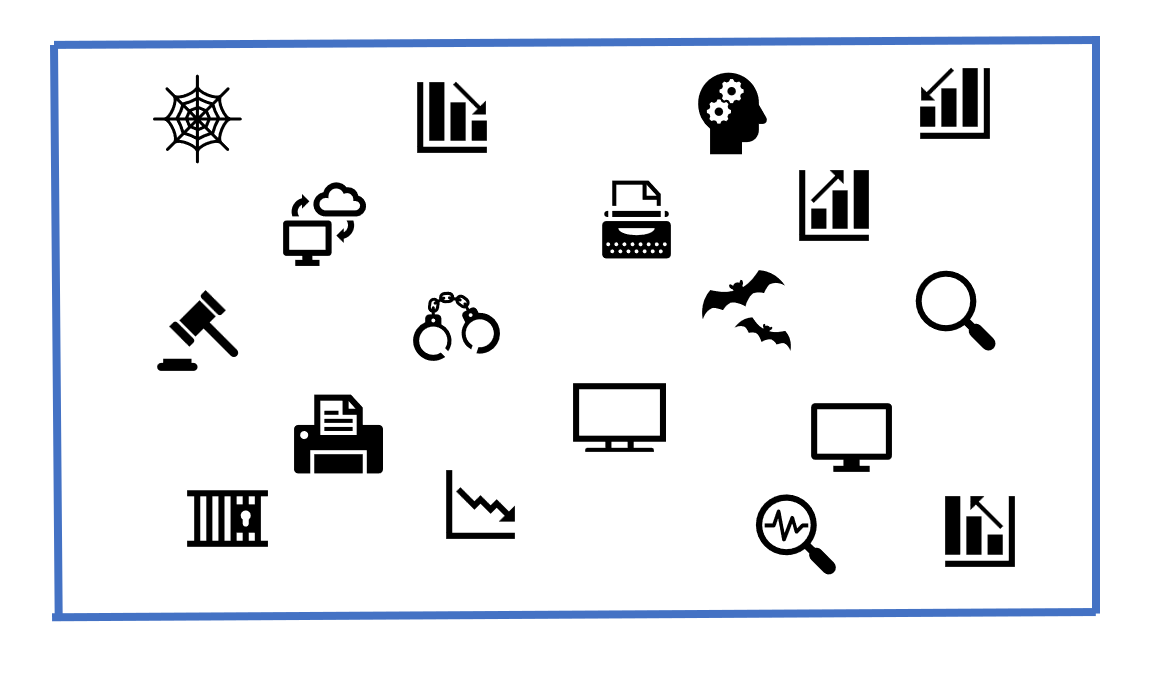
\includegraphics[scale=0.5]{template.jpg}
\caption{模板图片}
\end{figure}

\section{ORCA算法基本原理}
ORCA算法,英文全称是Optimal Reciprocal Collision Avoidance,最早在RVO的基础上演化而来,应用于时空交界下,移动式机器人相互碰撞避免场景。主要思想如下:一个任意移动物体的速度为$\symbf{v}$,包含有线速度linear和角速度angular,若将可能会发生碰撞的速度矢量看作一个集合,称之为$VO$(Velocity Obstacle)。如果把所有动态障碍物方向的速度排除在集合以外,可以得到关于无碰撞速度的集合,那么移动机器人在无碰撞的速度集合中取到的速度都不会发生碰撞,问题在于如何确定这个速度集合。本章在讨论动态避障问题时候,不对行人动态行为做深层次预测,将行人与其他动态障碍物做模式等效,也就是通过对当前速度的观测,假定在一段时间内,行人的运动模式不发生变化(实际情况下,园区内的行人运动方式的确有规可循),同时本文讨论的避障方法应用于多层级导航系统中,系统本身带有的避障算法可弥补因统一模型而带来的可能碰撞缺陷,因此本文讨论的前提是将行人与移动机器人的移动模式等效,且确认此种等效在本导航系统下不会出现系统性风险。


\subsection{ORCA在导航中应用的问题描述}
当移动机器人在环境中导航运动时,可行驶区域内一定范围出现另一动态障碍物,此时可虑让这二者不发生碰撞,将移动机器人和此障碍物归一化考虑,使用同一种模型去考虑不同的动态障碍物类型,以下统称为动态障碍物。对于任意的两个的动态障碍物A和B,速度障碍$VO^\tau_{A|B}$表示A相对于B的所有相对速度的集合,这个速度会导致A、B两个动态障碍物在$\tau$时刻内发生碰撞。

为描述的方便性以及公式引出的合理性,将导航过程中所有可能出现的动态障碍物都等效成圆模型,以便利对过程的推到。可定义为:
\begin{equation}
    D(\symbf{p},r) = \{\symbf{q}| ||\symbf{q}-\symbf{p}|| < r\}
\end{equation}
$D(\symbf{p},r)$表示圆心位置在$\symbf{p}$处的,半径为$r$的圆模型,$\symbf{q}$表示圆模型内的任意一点。

圆模型及A、B关于原点的对称圆模型如下所示:
\begin{figure}[ht]

    \centering
    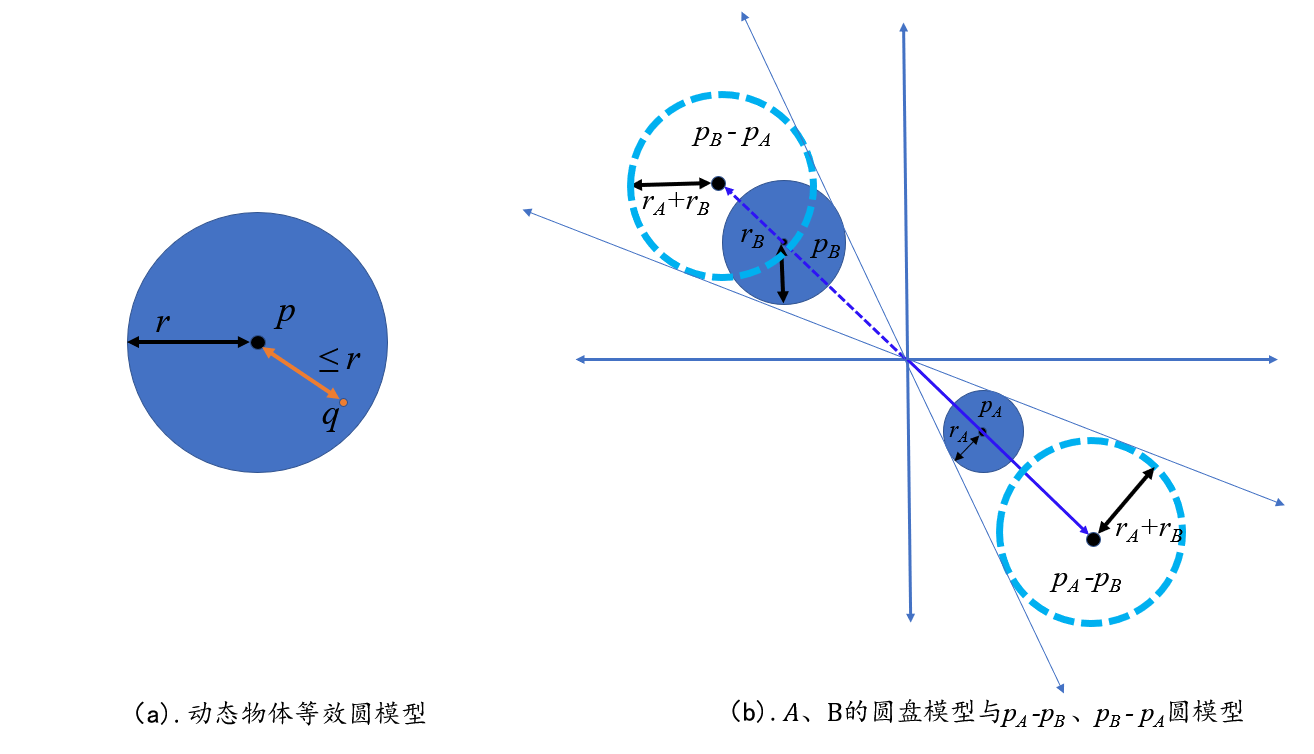
\includegraphics[scale=0.5]{circle_model.png}
    \caption{圆模型以及VO的分析图}
\end{figure}

据此可以用数学语言描述$VO^\tau_{A|B}$:
\begin{equation}
    VO^\tau_{A|B}  = \{\symbf{v}| \exists t \in [0, \tau]::t \symbf{v} \in D(\symbf{p}_B - \symbf{p}_A, r_A + r_B)\}
\end{equation}

速度障碍可以由几何表示,如图:
\begin{figure}[ht]

    \centering
    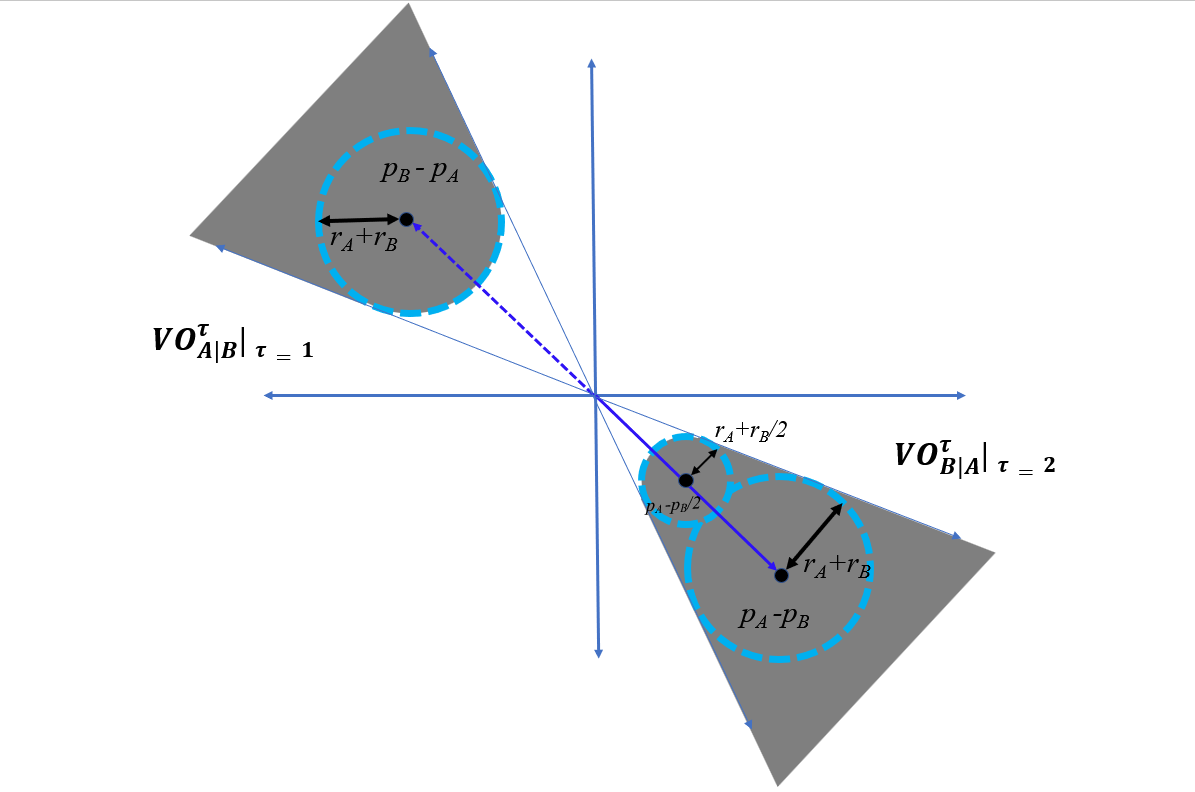
\includegraphics[scale=0.5]{circleCA_model.png}
    \caption{$VO^\tau_{A|B}$与$VO^\tau_{B|A}$}
\end{figure}
$VO^\tau_{A|B}$与$VO^\tau_{B|A}$在$\tau$相同时是关于原点对称的截断锥形,从图4.2(b)可知$D(\symbf{p_B-p_A},r_A+r_B)$与$D(\symbf{p_A-p_B},r_A+r_B)$也是关于原点对称的。
对上图中$VO^\tau_{B|A}|_{\tau=2}$可用物理描述解释为:若B相对于A的速度处于图4.3的灰色区域之中,那么在时间窗口$\tau=2$之前的某个时刻,A、B之间将发生碰撞。以上是速度障碍的最直观解释。


由此特例推广开来,对于A、B两个物体的速度$\symbf{v}_A$、$\symbf{v}_B$,如果A、B在$\tau$时刻内继续以当前速度运动,那么,A、B必将在某个时刻发生碰撞。此过程可以等效描述为:
\begin{equation}
    \begin{aligned}
        &\symbf{v}_A - \symbf{v}_B \in  VO^\tau_{A|B} \\
        &or:\\
        &\symbf{v}_B - \symbf{v}_A \in  VO^\tau_{B|A}
    \end{aligned}
\end{equation}

如果从这个角度出发,要让A、B在一定时间内不发生互相碰撞,可以通过:$\symbf{v}_A$ - $\symbf{v}_B$ $\notin$  $VO^\tau_{A|B}$来完成。那么可以至少保证在$\tau$时刻内,A、B两个物体互相之间无碰撞。由此可得,当B在集合$V_B$中选择速度$\symbf{v}_B$,即$\symbf{v}_B$ $\in$ $V_B$,对于A物体来说,若要两者不发生碰撞,相当于
\begin{equation}
    \symbf{v}_A \notin  VO^\tau_{A|B} \oplus \symbf{v}_B
\end{equation}

式中$\oplus$表示明可夫斯基和,即集合的并集关系。由$\symbf{v}_A$的取值范围,可以引出A物体相对于B的避碰速度集(Collision Avoidance):
 \begin{equation}
    CA^\tau_{A|B}(V_B) =  \{ v|\symbf{v} \notin VO^\tau_{A|B} \oplus \symbf{v}_B\}
\end{equation}
也即 $\symbf{v}_A$ $\in$ $CA^\tau_{A|B}(V_B)$时,A、B在$\tau$时间内不会发生碰撞。

$CA^\tau_{A|B}(V_B)$可用几何图形解释为如图:
\begin{figure}[ht]
    \centering
    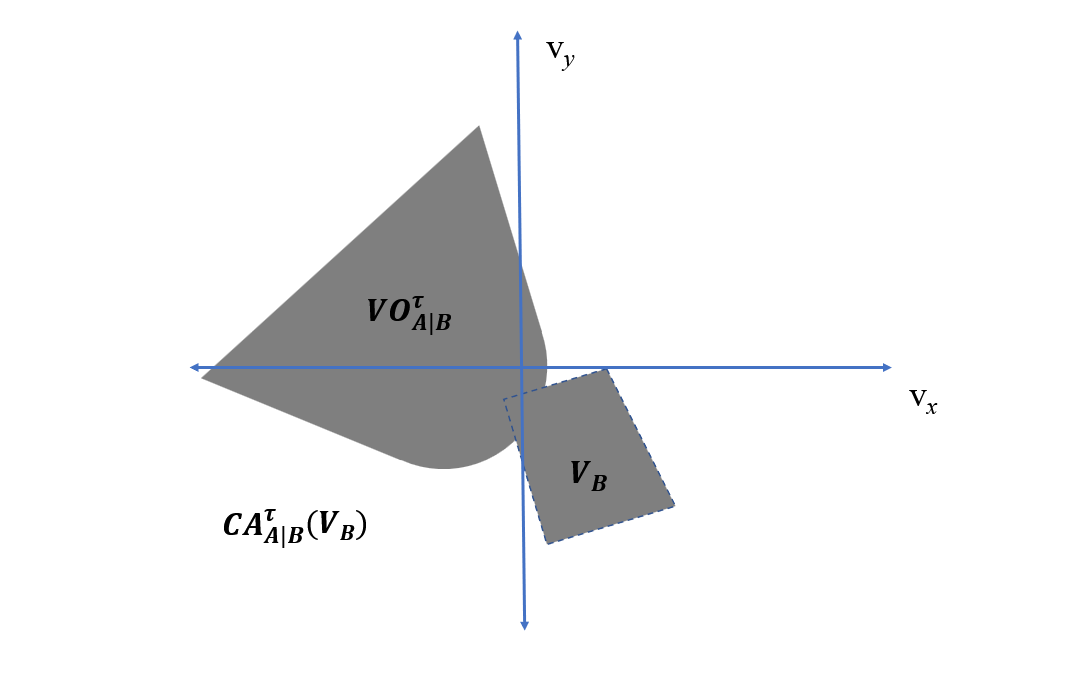
\includegraphics[scale=0.5]{circle_CA.png}
    \caption{A相对于B的避碰速度集几何解释}
\end{figure}
图4中所有灰色之外均为避碰速度。

定义集合为属于A、B物体的避碰速度集合的子集,当两个子集分别和其父集合重合时,此时的$V_A$ 、$V_B$称为最大速度避碰集合。

此时如果有两个任意速度集合$V_A$ 、$V_B$,且这两个速度集合又是$CA^\tau_{A|B}(V_B)$、$CA^\tau_{B|A}(V_A)$的子集,那么称这两个集合RCA(reciprocally collision-
avoiding )集。基于上述叙述,在选择避碰速度集合时,希望为A、B直接在$CA^\tau_{A|B}(V_B)$、$CA^\tau_{A|B}(V_B)$ 中选择速度,以保证A、B在时间窗口$\tau$内不会发生碰撞并且可选择的速度最多。


在本文搭建的导航系统下, 移动机器人在接受了目标点之后,会有一个最优的速度接近目标点,
那么按照上述推理,分别将机器人与人都视作圆盘模型,则希望找到一个集合最大限度地“接近”导航系统当前时刻需要地最优速度$v^{opt}$,将这个集合定义为ORCA集合。若两个物体分别是仍记作A、B,ORCA则记作$ORCA^\tau_{A|B}$、$ORCA^\tau_{B|A}$。



\subsection{ORCA的求解}
求解ORCA的过程不需要通过大量的非线性计算,而可以通过集合构造求解的方式进行,如图:
\begin{figure}[ht]
    \centering
    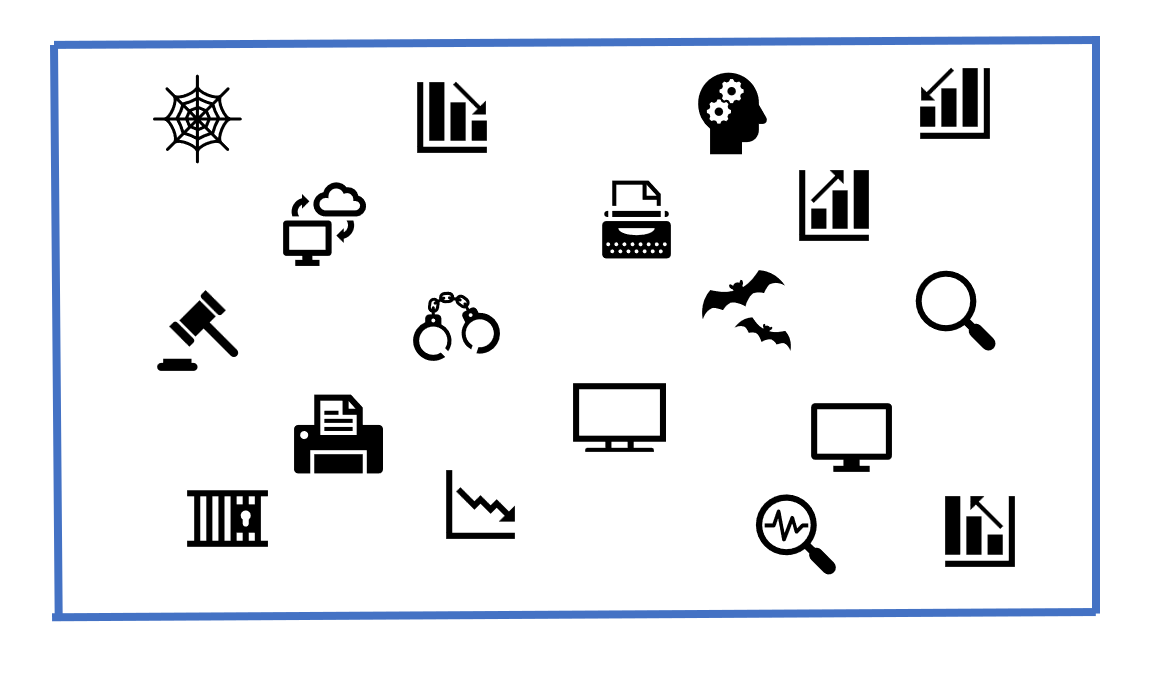
\includegraphics[scale=0.5]{template.jpg}
    \caption{模板图片}
\end{figure}
在此刻假设移动机器人分别采用最优速度$\symbf{v}_A^{opt}$、$\symbf{v}_B^{opt}$,且这会导致A、B之间产生碰撞。即:
\begin{equation}
    \symbf{v}_A^{opt} - \symbf{v}_B^{opt} \in  VO^\tau_{A|B}
\end{equation}
而$\symbf{u}$为$\symbf{v}_A^{opt}$-$\symbf{v}_B^{opt}$到速度障碍边界上最近的点的向量,则$\symbf{u}$是A、B在时间窗口$\tau$内避免碰撞所需要做出的相对速度的最小变化,即:
\begin{equation}
    \symbf{u} = ( \mathop{\arg\min}\limits_{\symbf{v} \in \partial VO^\tau_{A|B}} || \symbf{v} - (\symbf{v}_A^{opt}-\symbf{v}_B^{opt})||) - (\symbf{v}_A^{opt}-\symbf{v}_B^{opt})
\end{equation}
$\symbf{n}$为速度边界处在点$\symbf{v}_A^{opt}$-$\symbf{v}_B^{opt}$ + $\symbf{u}$的法线。
则$\symbf{u}$是A、B在时间窗口$\tau$做出碰撞避免所需的最小相对速度变化。一般情况下,在多机器人系统的避障策略中,以对半分摊最小相对速度变化的方式计算ORCA,即:
\begin{equation}
    ORCA^\tau_{A|B} = \{\symbf{v} | (\symbf{v}-(v_A^{opt} + \frac{1}{2}\symbf{u}))\cdot\symbf{n} \geq 0\}
\end{equation}

在本导航系统的考虑中,为了安全准则考虑,假设行人、其他车辆等障碍物对速度的调节量降低,不以常用的对半分摊最小相对速度变化的方式考量,那么对于选定的代理机器人而言:
\begin{equation}
    ORCA^\tau_{A|B} = \{\symbf{v} | (\symbf{v}-(v_A^{opt} + \frac{3}{4}\symbf{u}))\cdot\symbf{n} \geq 0\}
\end{equation}

% !!!!!!!!!!!


求解图中的$\symbf{u}$,有表达式:
\begin{equation}
    \symbf{u} = ( \mathop{\arg\min}\limits_{\symbf{v} \in \partial VO^\tau_{A|B}} || \symbf{v} - (\symbf{v}_A^{opt}-\symbf{v}_B^{opt})||) - (\symbf{v}_A^{opt}-\symbf{v}_B^{opt})
\end{equation}
可以解释为假设A和B的自适应速度分别为$v_A^{opt}$、$v_B^{opt}$,那么A、B会碰撞,则
$\symbf{v}_A^{opt}$ - $\symbf{v}_B^{opt}$ $\in$  $\symbf{VO}^\tau_{A|B}$,$\symbf{u}$
是以$\symbf{v}_A^{opt}$ - $\symbf{v}_B^{opt}$为起点,指向最接近$\symbf{ORCA}^\tau_{A|B}$
边界的点的向量。


求解图中的$\symbf{n}$,有表达式:
\begin{equation}
    \symbf{n} = (v_A^{opt}-v_B^{opt}) + \symbf{u}
\end{equation}
表达式可以解释为$\symbf{n}$是以$\symbf{VO}^\tau_{A|B}$的边界上的点($v_A^{opt}$-$v_B^{opt}$)+$\symbf{u}$
为起点,向外延伸的法线。


求解$\symbf{ORCA}^\tau_{A|B}$,有表达式:
\begin{equation}
    \symbf{ORCA}^\tau_{A|B} = \{\symbf{v} | (\symbf{v}-(v_A^{opt} + \frac{1}{2}\symbf{u}))\cdot\symbf{n} \geq 0\}
\end{equation}
此关键表达式被解释为: $\symbf{ORCA}^\tau_{A|B}$是一条被直线分割开的一个半平面集合,这个半平面
集合为$\symbf{n}$指向的一侧。其中这条直线垂直于$\symbf{u}$,且穿过点$v_A^{opt}$ + $\frac{1}{2}$,
由两点确定一条直线。






\subsection{多个机器人碰撞的情况}

上述情况针对于仅有两个移动机器人的碰撞情况,当实际情况中出现多个机器人时,需要在确定了一个主题之后,对其他所有的移动机器人归为一类,都视为当前机器人A的B。即对于机器人A的所有B有
\begin{equation}
    \symbf{ORCA}^\tau_A = D(0, v_A^{max}) \cap (\mathop{\bigcap }\limits_{A \neq B}\symbf{ORCA}^\tau_{A|B})
\end{equation}

也就是说此时 $\symbf{ORCA}^\tau_A$是机器人A相对于其他任意机器人B,以它的最大速度$v_A^{max}$为半径的圆与其他所有B的ORCA的交集。而后机器人在集合允许的速度范围内选择最接近其设定的最优速度$v_A^{pref}$的
新速度$v_A^{new}$:
\begin{equation}
    v_A^{new} = \mathop{\arg\min}\limits_{\symbf{v} \in \symbf{VO}^\tau_A}||v- v_A^{pref}||
\end{equation}

此时求得的速度便是允许的速度集合中最接近最优速度的速度值,机器人的位置便可以旧的位置$p_A$加上速度乘以时间求得。


\section{基于ORCA的系统级避障策略}
第3章对系统方法描述中介绍了系统运行过程中使用点云点检测和体素网格方式进行近距离范围的避障策略。此避障方法简单而有效,在静态场景以及很少动态物体出现的区域时候表现良好,但应对多动态区域时会使得整个规划模块混乱。因此在穿越多动态区域时,需要对此方法进行改良,并且与ORCA的线程结合。两者结合的有点至少有两个:1.保证移动机器人穿越多动态区域时具有优秀的规划与避障能力;2.将ORCA原本的静态障碍物规划过程免去,只需要计算对应的动态障碍物速度障碍即可,减少了系统的计算量。

\subsection{多动态区域的移动物体观测与速度计算}
要开展ORCA的计算,首先需要对考虑范围内的移动障碍物进行速度观测或估计。本文第三章3.3节已经详细介绍了对周边障碍物的分割与聚类过程,可以得到需要观测环境内的动态障碍物的实例分割。接下来对相应的实例进行简单地速度观测。

此处借助高层导航构建地先验栅格地图,此地图以园区内图书馆某处为坐标系原点建立,故可以用以下示意图表示动态障碍物的占据与移动趋势。本文进行ORCA避障的前提不对实例中每个点进行分析,而是对占据的栅格进行动态占据的方式分析被占据栅格的移动趋势。移动机器人在全局地图上的移动仅限于可行驶区域,故首先提取可行驶区域上的动态障碍物点云信息。

上述得到分割后的实例之后,确定可行驶区域上的动态障碍物方法是通过高度阈值进行判断,判断的方法基于动态物体(例如车、行人等)与地面有接触。上一章中已经对地面点和可行驶区域以及移动机器人周围的实例对象进行了分割介绍。本文此部分更加着重于对动态障碍物的分辨和移动趋势计算。
将此刻移动机器人附近的可行驶区域与之前高层导航方法中分割出的地面点进行对比,即可得到此时可行驶区域上新出现的障碍物点云,由于园区场景内静态障碍物位置与区域基本不发生变化,故新多出的障碍物点云即可认为是移动障碍物。对移动障碍物点云的最高点高度值max\_height记录并且记录此刻点云在栅格地图上所占据的栅格索引值index,设置点云的标签为:
\begin{equation}
    label = \alpha * max_height + \beta * index
\end{equation}

其中label是对点云的记录标签,$\alpha $、$\gamma $分别代表点云高度最高值和索引值在标签中所占的比例系数。在高动态场景下,$\alpha $所占比例应当适当调高,将关注重点放在动态物体的本身特质上。
对场景内可行驶区域上的所有动态点云建立标签集,当下一次扫描来临时,对扫描得到标签集进行阈值搜索,匹配两次扫描的标签集。认为当前扫描的标签集是动态障碍物两次扫描的对应位置变化。接下来计算相应物体的移动速度。

示意图如下所示:

\begin{figure}[ht]
    \centering
    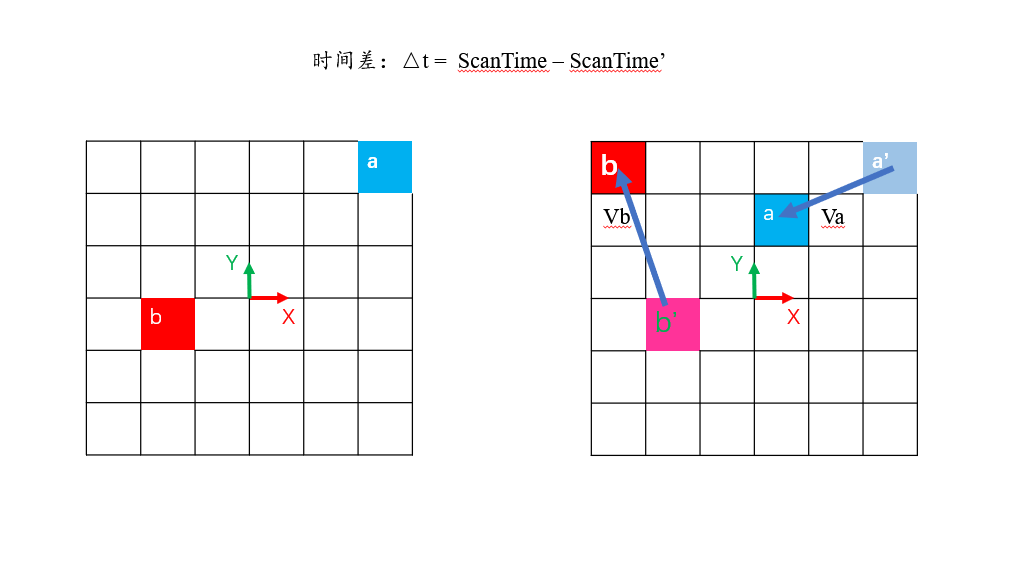
\includegraphics[scale=0.5]{voxel_move.png}
    \caption{全局栅格地图与动态障碍物的占据与移动趋势}
\end{figure}
移动障碍物在全局栅格地图上的占据位置随时间发生变化,任意一个移动障碍物的速度可以估算为:
\begin{equation}
    V =  \frac{\sqrt{(Voxela'.y - Voxela.y)^2 + (Voxela'.x - Voxela.x)^2} }{\varDelta t}
\end{equation}

Voxela'.y、Voxela'.x、Voxela.y、Voxela.x分别表示扫描时刻ScanTime'和ScanTime时刻被占据方格中心的坐标值;$\varDelta t$是两次扫描的时间间隔。速度的方向即为图中箭头所示的方向,图中的坐标系指的是校园中选定的全局坐标系的位置。
至此,移动机器人周围的动态物体的移动速度即可通过观测得到。可以开始下一步的速度障碍的计算。


\subsection{ORCA与系统的结合方案}
在ORCA模块不启动情况下,移动机器人的导航系统会根据当前的目标点在局部规划时给出相应的路径,即运动元路径组中的某一条。ORCA避障模块启动后,会将当前路径组中选定的路径的方向和速度大小作为参考值即前面原理中提到的$V_pref$。离线运动元路径组是以点的形式存于txt文件中,并在每次程序运行时启动并读取存于相应的vector容器中。
由于离线路径组的转向角度并不同于路径组的路径方向,故需要对路径组的路径速度方向计算。
离线路径组的速度方向的计算方式如下图所示:

\begin{figure}[ht]
    \centering
    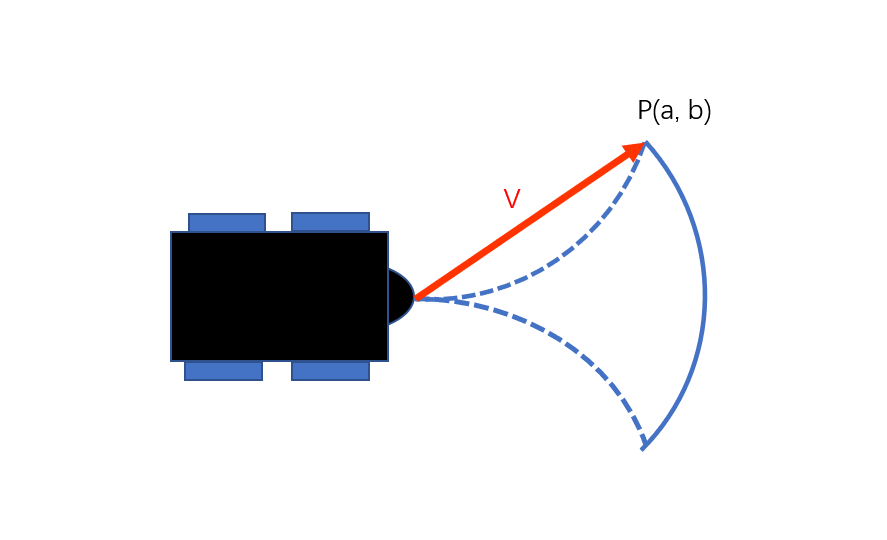
\includegraphics[scale=0.5]{path_atan2.png}
    \caption{离线运动元路径组的速度方向计算}
\end{figure}

图中运动元在路径终点处的点为P, 坐标值分别为a、b。那么移动机器人选择此条路径的移动速度方向即为:
\begin{equation}
    V_\theta = atan2(b ,a) * 180 / \pi 
\end{equation}
此速度方向即为ORCA计算速度原理中$V_{pref}$的速度方向,大小则直接读取相应的路径对应的默认速度大小。

然后根据上述的观测,确定一定范围内的可行驶区域中存在的动态障碍物数量,据此通过ORCA库中的Agent::computeNewVelocity()函数计算出上述计算原理中的$v_{new}$,原始的ORCA算法在此处即可完成计算,并且将$v_{new}$输入给机器人系统执行运动。但此处计算出的速度是将机器人当作圆盘模型构建的,拥有360°无死角的全方位原地转向能力,故此速度在实际移动机器人底盘上无法执行。
本文提出的算法在速度计算之初将模型当作圆模型进行处理,也就是说,得到的速度$v_{new}$是阿克曼模型中心位置所需要进行运动的速度和方向,但是很明显,阿克曼模型中心并不能随心所欲地按照$v_{new}$给出的速度大小和方向运动,因此必须得在得到计算结果后对速度$v_{new}$与阿克曼的模型进行适配。计算得到$v_{new}$之后做出下处理:

(1).若检测到移动机器人的位置已经在终点处,则令速度为0,停止规划;

(2).计算当前移动机器人的朝向yaw角度与$v_{new}$之间的角度差值$\varDelta\theta$ ,若速度角度差$\varDelta \theta$在阈值之外,也就是说移动机器人不可以通过走直线来接近局部目标点,同时表示移动机器人在目前朝向下不可能向着局部目标点方向出发,于是低速调整速度方向:取$\varDelta\theta$符号sign,使用阿克曼模型的最大转向角度向着偏差方向慢速调整速度方向;

(3).若$\varDelta \theta$在转向阈值之内,表示机器人运动元路径组的覆盖方向包含有$v_{new}$的方向,并且此时移动机器人没有到达目标点,需要将此速度$v_{new}$适配到阿克曼底盘上,因ORCA计算过程是将速度转化成向量及其投影简化计算,其计算出的$v_{new}$以向量形式表示,在x、y方向上的速度分量分别是($v_{new}.x$、$v_{new}.y$),不能直接使用,需要转化成线速度(推进速度)以及角速度的形式,才可成为阿克曼底盘可用的速度:


    必须明确的是在本实验平台下,阿克曼底盘移动机器人按照$v_{new}$进行移动,指的是移动机器人在路径组的group中的第一段路径终点位置与路径起点的连线方向与$v_{new}$一致。

    首先需要确定移动机器人底盘的角速度:
    当前时刻移动机器人在全局坐标系下的朝向为$\theta$,且当前所需要的速度方向为atan2($v_{new}.y$, $v_{new}.x$),根据上述介绍的离线路径组的速度方向,选择与$v_{new}$速度方向最接近的一条路径,通过此路径对应的索引查询到此路径本身带有的角速度信息$angular$。

    确定要走的路径之后,接下来确定线速度$v_linear$的大小:
    在任意时刻,沿着选定的运动元路径行驶时,运动机器人的当前线速度为$v_linear$,移动机器人的朝向与$v_{new}$的夹角为$ \varphi$,如图所示:
    \begin{figure}[ht]
        \centering
        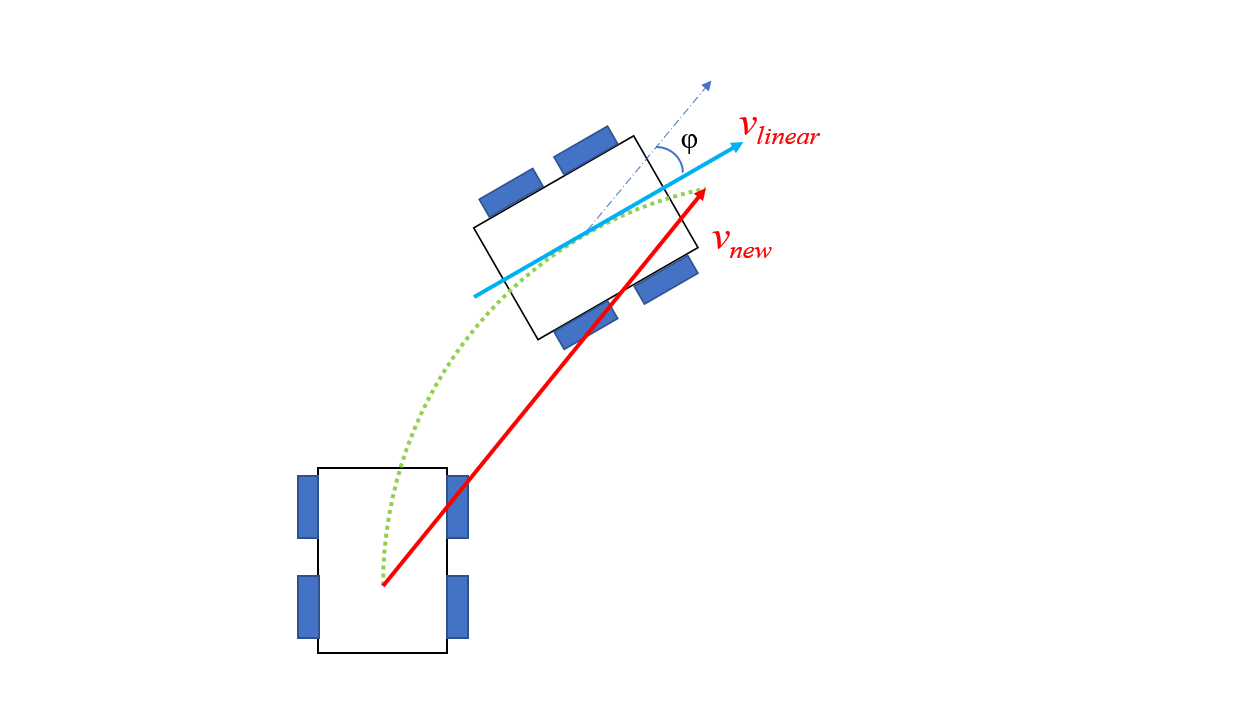
\includegraphics[scale=0.5]{ackerman_diff2.png}
        \caption{阿克曼模型的速度方向与大小等效方式}
    \end{figure}
    有等式:
    \begin{equation}
        v_{linear}  = \sqrt{(v_{new}.x)^2 + (v_{new}.y)^2} {\cos\varphi}^-1 
    \end{equation}
    $v_linear$即为发送给阿克曼底盘的线速度(推进速度)。

上述过程最终可以得到相应的最终速度, $v_linear$和$angular$这两者组合成的的速度便可以输入回规划系统并传给运动控制模块进行机器人运动控制。

% \section{次选等效方案}
%     很糟糕的一点是,阿克曼模型不可以直接向着转向阈值外的区域转向,并且前轮的线速度和角速度容易计算,但是前后轮的线速度由于前轮目前存在的转向,与实际情况下阿克曼模型的推进速度并不相等。于是对阿克曼模型进行等效。

%     首先需要将阿克曼车辆模型等效成一个有转向阈值的前轮(类似于有转向限制的差速底盘)和跟随前轮移动的固定后轮模型,如下图所示:
%     \begin{figure}[ht]
%         \centering
%         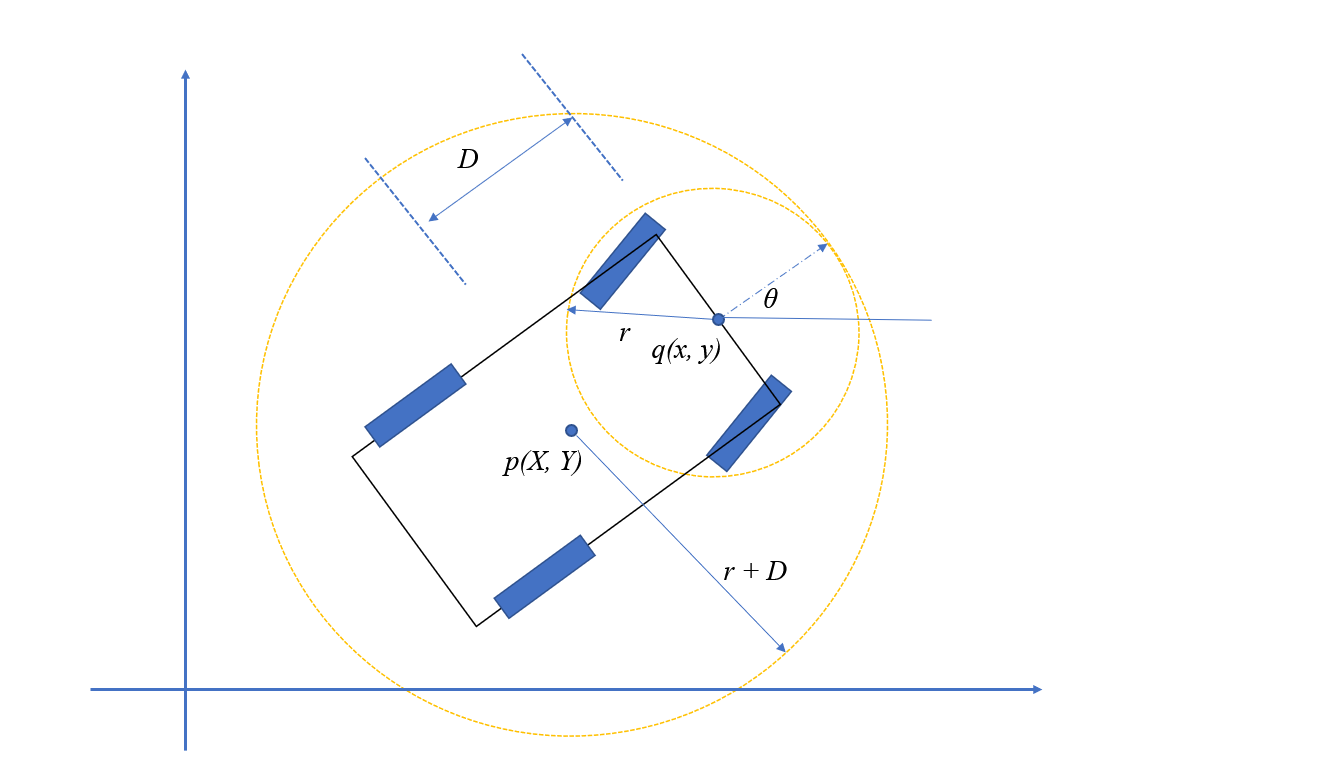
\includegraphics[scale=0.5]{ackerman_diff.png}
%         \caption{阿克曼模型的等效}
%     \end{figure}


%     阿克曼底盘的移动机器人的中心位置在P(X, Y)处,但糟糕的是这个点的位置并不可控,也就是说此点不能通过给定底盘相应的速度方向和大小来确定其下一时刻的位置。
%     于是本文将阿克曼等效为头部的圆模型,前部分的圆模型可以通过给定确切的速度方向和大小进行控制,这非常符合ORCA计算出的$v_{new}$的特点,有方向和大小即可。

%     但这样等效具有极大的弊端,等效出的前轮中心并不能代表移动机器人的整车位置。而且发送速度要求是整体车身的角速度和线速度,只考虑前轮明显不可行。如何在确定前两轮的移动速度和方向的前提下,得到车身整体的线速度和角速度,则是下面考虑的问题。

%     \textcolor{red}{得到的v new需要换算成线速度和角速度,目前是(vx, vy)的形式}
%     前轮等效出的有转向阈值的圆盘模型的轮速设置为$v_{front}$,
%     半径为R,则整体阿克曼模型的等效半径 R = r - D;根据阿克曼底盘目前的朝向$\theta $,可以得出:
%     \begin{equation}
%         \begin{aligned}
%             X = x - D \cos \theta \\
%             Y = y - D \sin \theta 
%         \end{aligned}
%     \end{equation}

%     考虑到此刻等效出的前轮圆盘模型中,q(x, y)以及此刻的朝向
%     \begin{equation}
%         \left[\begin{array}{c}
%         \dot{x} \\
%         \dot{y} \\
%         \dot{\theta} 
%         \end{array}\right]=\left[\begin{array}{c}
%         \cos \theta \\
%         \sin \theta \\
%         \tan \theta / L 
%         \end{array}\right] v_{1}
%     \end{equation}
%     其中L表示轮距,$v_1$表示阿克曼底盘的线速度。

%     联立上述两式,可得:
%     \begin{equation}
%         \begin{aligned}
%             \dot{X} = v_1\cos\theta + v_1D\sin\theta\tan{\frac{\theta}{L}} \\
%             \dot{Y} = v_1\sin\theta - v_1D\cos\theta\tan{\frac{\theta}{L}}
%         \end{aligned}
%     \end{equation}

%     那么此刻“有效中心”位置的速度($\dot{X}$, $\dot{Y}$),可以得到,如此便可以反求出应有的推进速度,即发送给底盘执行所需要的速度$v_1$。









\section{动态避障系统的仿真实验}
实验环境:Ubuntu操作系统, ROS机器人操作系统,构建阿克曼运动学模型于rviz中,并通过stage\_ros内部传递多个机器人之间的速度与位置信息。

实验设置:该实验通过rviz与stage\_ros作为实验环境,通过xarco文件构建阿克曼机器人模型,并将模型置于rviz界面中,通过stage\_ros作为信息状态的处理中心,机器人状态的共享是通过使用ROS中的机器人状态发布器(robot\_state\_publisher)和关节状态发布器(joint\_state\_publisher)来实现的。

首先,在每个机器人的命名空间中,启动一个 robot\_state\_publisher 节点和一个 joint\_state\_publisher 节点。robot\_state\_publisher 节点订阅机器人的 URDF 模型和机器人的关节状态,然后将机器人状态发布到 /tf 主题上。joint\_state\_publisher 节点从 /joint\_states 主题订阅关节状态,并将其转换为 /tf 主题上的机器人状态。

然后,在每个机器人的命名空间中,启动一个 move\_server 节点和一个 move\_client 节点。move\_server 节点负责处理机器人的运动控制,例如机器人的速度控制和路径规划。move\_client 节点是一个简单的命令行工具,用于向 move\_server 发送命令控制机器人运动。

在最后一部分的 static\_transform\_publisher 节点中,发布一个静态的 TF 变换,将机器人的 /map 坐标系和 /odom 坐标系对应起来。这样就可以在 rviz 中显示机器人在地图上的位置。由于机器人状态发布器和静态 TF 发布器发布的是相同的机器人状态,因此在 rviz 中看到的机器人位置和在 Stage\_ros 中看到的机器人位置是相同的,也可以通过改变stage\_ros中机器人的状态来影响rviz中机器人的状态。

实验中所使用到的栅格地图环境使用“map\_sever”服务器进行加载,主要加载的是无障碍物的栅格地图区域,目的是执行ORCA的动态避障效果。此处实验不考虑静态障碍物,此部分已经在第3章中详细叙述并且实验证明。

rviz下建立的阿克曼机器人模型如下图所示:
\begin{figure}[ht]
    \centering
    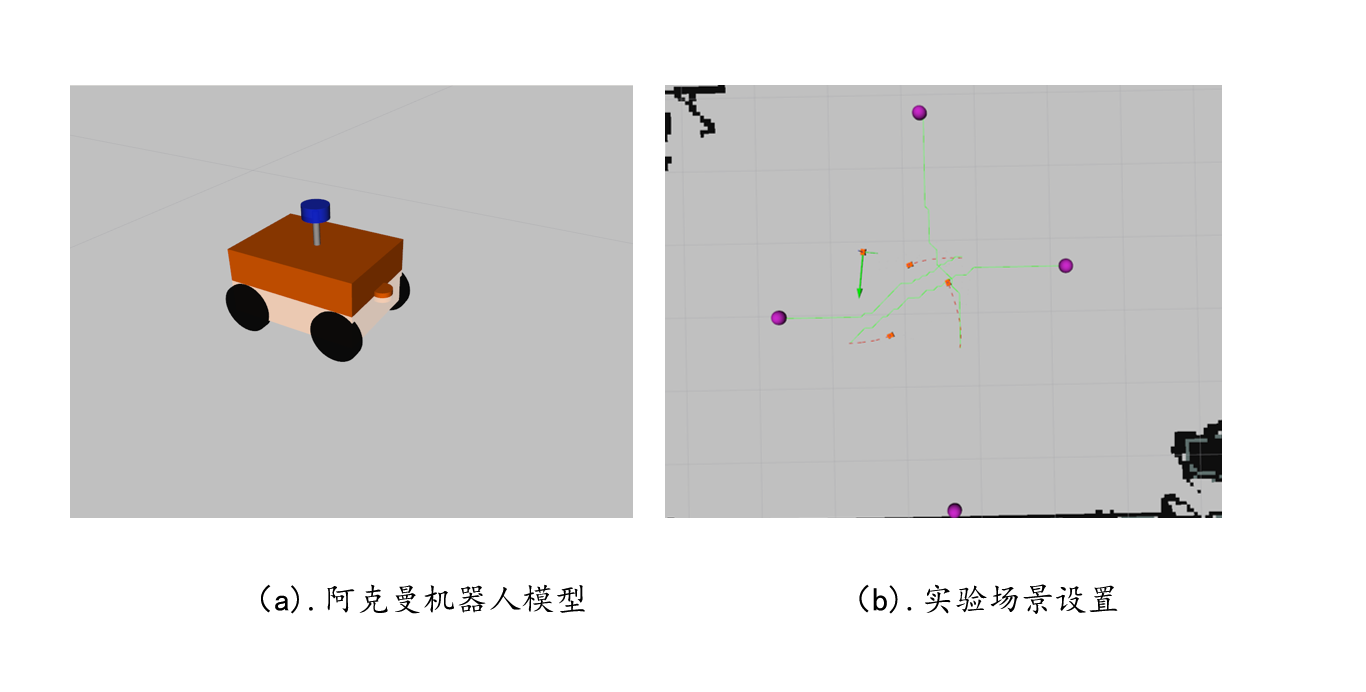
\includegraphics[scale=0.5]{model_scene.png}
    \caption{仿真环境中的阿克曼模型和场景}
\end{figure}

阿克曼模型依据实验室移动移动机器人的外形作为设计参考,具备底盘、三维激光雷达和2D激光雷达。场景中紫色球部分为实验为移动过程中移动机器人需要到达的指定目标点,通过指定目标点的形式模仿实际应用中不同动态物体向着不同方向和趋势移动的过程。绿色实线是在栅格地图上使用A*算法规划处的路径,目的是按照移动机器人的导航系统方式设置高层的规划方案。红色部分虚线是各个动态障碍物实际运行中产生的轨迹。绿色虚线部分为选定主要研究对象的轨迹,并且研究对象还会在车身部分增添相应base\_link坐标系,并通过绿色箭头部分(即其odometry)来研究其各个时刻对应的速度方向。

实验假定场景中存在的障碍物都以阿克曼模型为约束,并选定一个移动移动机器人作为主要研究对象,观察其轨迹。如此设置实验的好处是,虽然只选定了一个机器人作为研究对象,但是其他机器人使用的是与选定代理一样的算法,可以最大程度模拟现实应用中出现的各种遭遇情况,并且选定的代理亦可作为其他实验对象的动态障碍物,多点研究,模拟情况种类丰富。并且由于实际使用中,路径的规划是本身自带静态避障的,故本仿真实验可以使用车模型一定程度替代实际场景上遭遇到的行人等物体。

实验设计主要分为两个类别、两种场景:1. 4或者8动态障碍物的相向对穿实验、同向争点实验以及同向穿插实验。通过这三个实验分别验证现实场景中可能出现的几种穿越动态区域的情况。考虑到仿真环境地地图栅格分辨率为0.05m,且环境中设置的机器人最大速度为0.3m/s,故本文实验所取得时间窗口大小$\tau$ = 3s,即图中移动机器人在移动两个大栅格的情况下都不会发生与其他机器人的碰撞,这样取值是十分合理且具有代表性的。 

\subsection{实验一:4动态障碍物遭遇实验}
实验在同一无静态障碍物区域放置4个动态物体,此4物体即互相做障碍物也单独可称为研究主体。

\subsubsection{对穿实验}
实验中选定的ORCA算法所需要的$V\_opt$是5.3节局部规划器规划出的运动元路径所指向的速度方向。故此种选法是一种激进的$V\_opt$选择策略。


\begin{figure}[ht]
    \centering
    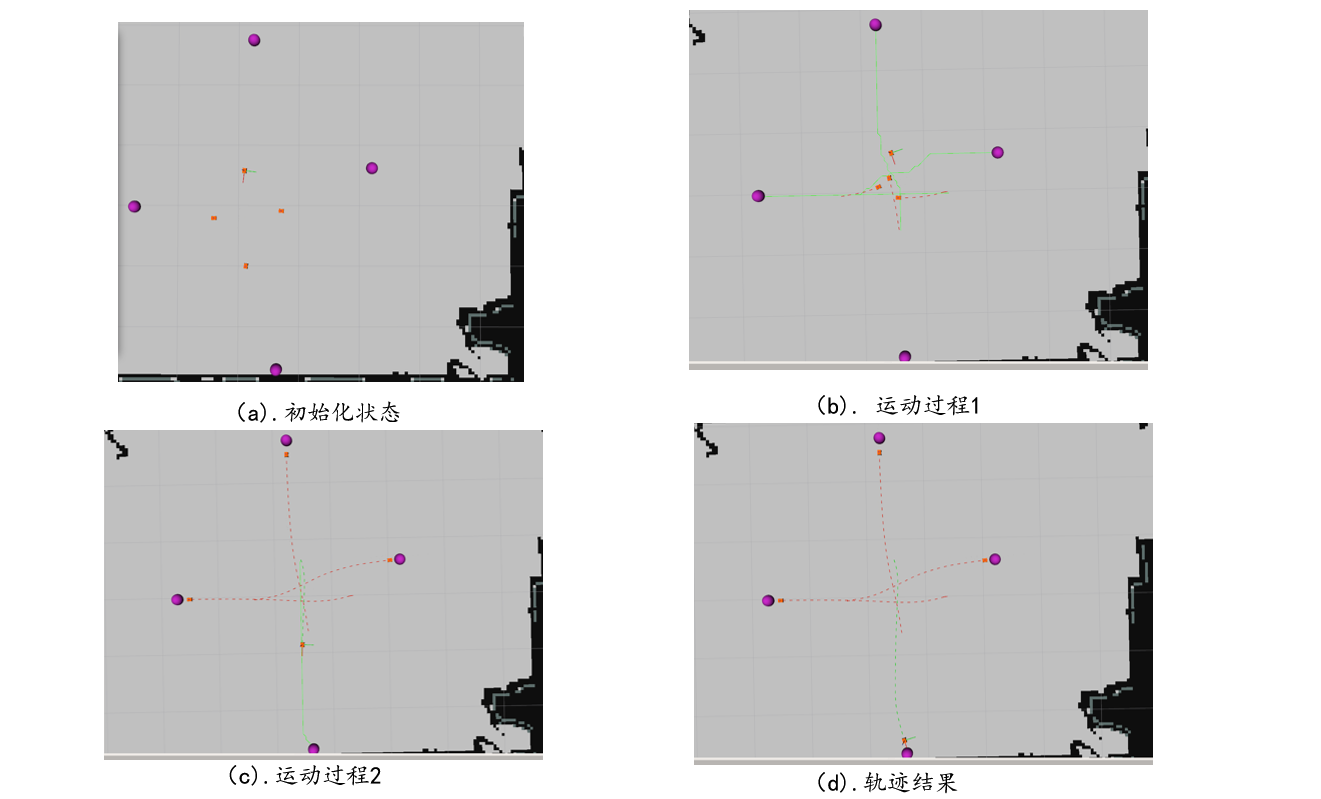
\includegraphics[scale=0.5]{orca_4_1.png}
    \caption{4动态障碍物对穿实验1}
\end{figure}


上述图片展示了各动态障碍物面向终点并且对穿的过程,可以看到在中心的交汇处,由于ORCA算法对速度的调整,轨迹出现了一定程度的改变。
下面展示更多情况下的实验室结果并配以选定的对象的速度调整图像,下图中不再展示运行过程,尽量多地展示实验结果:
\begin{figure}[ht]
    \centering
    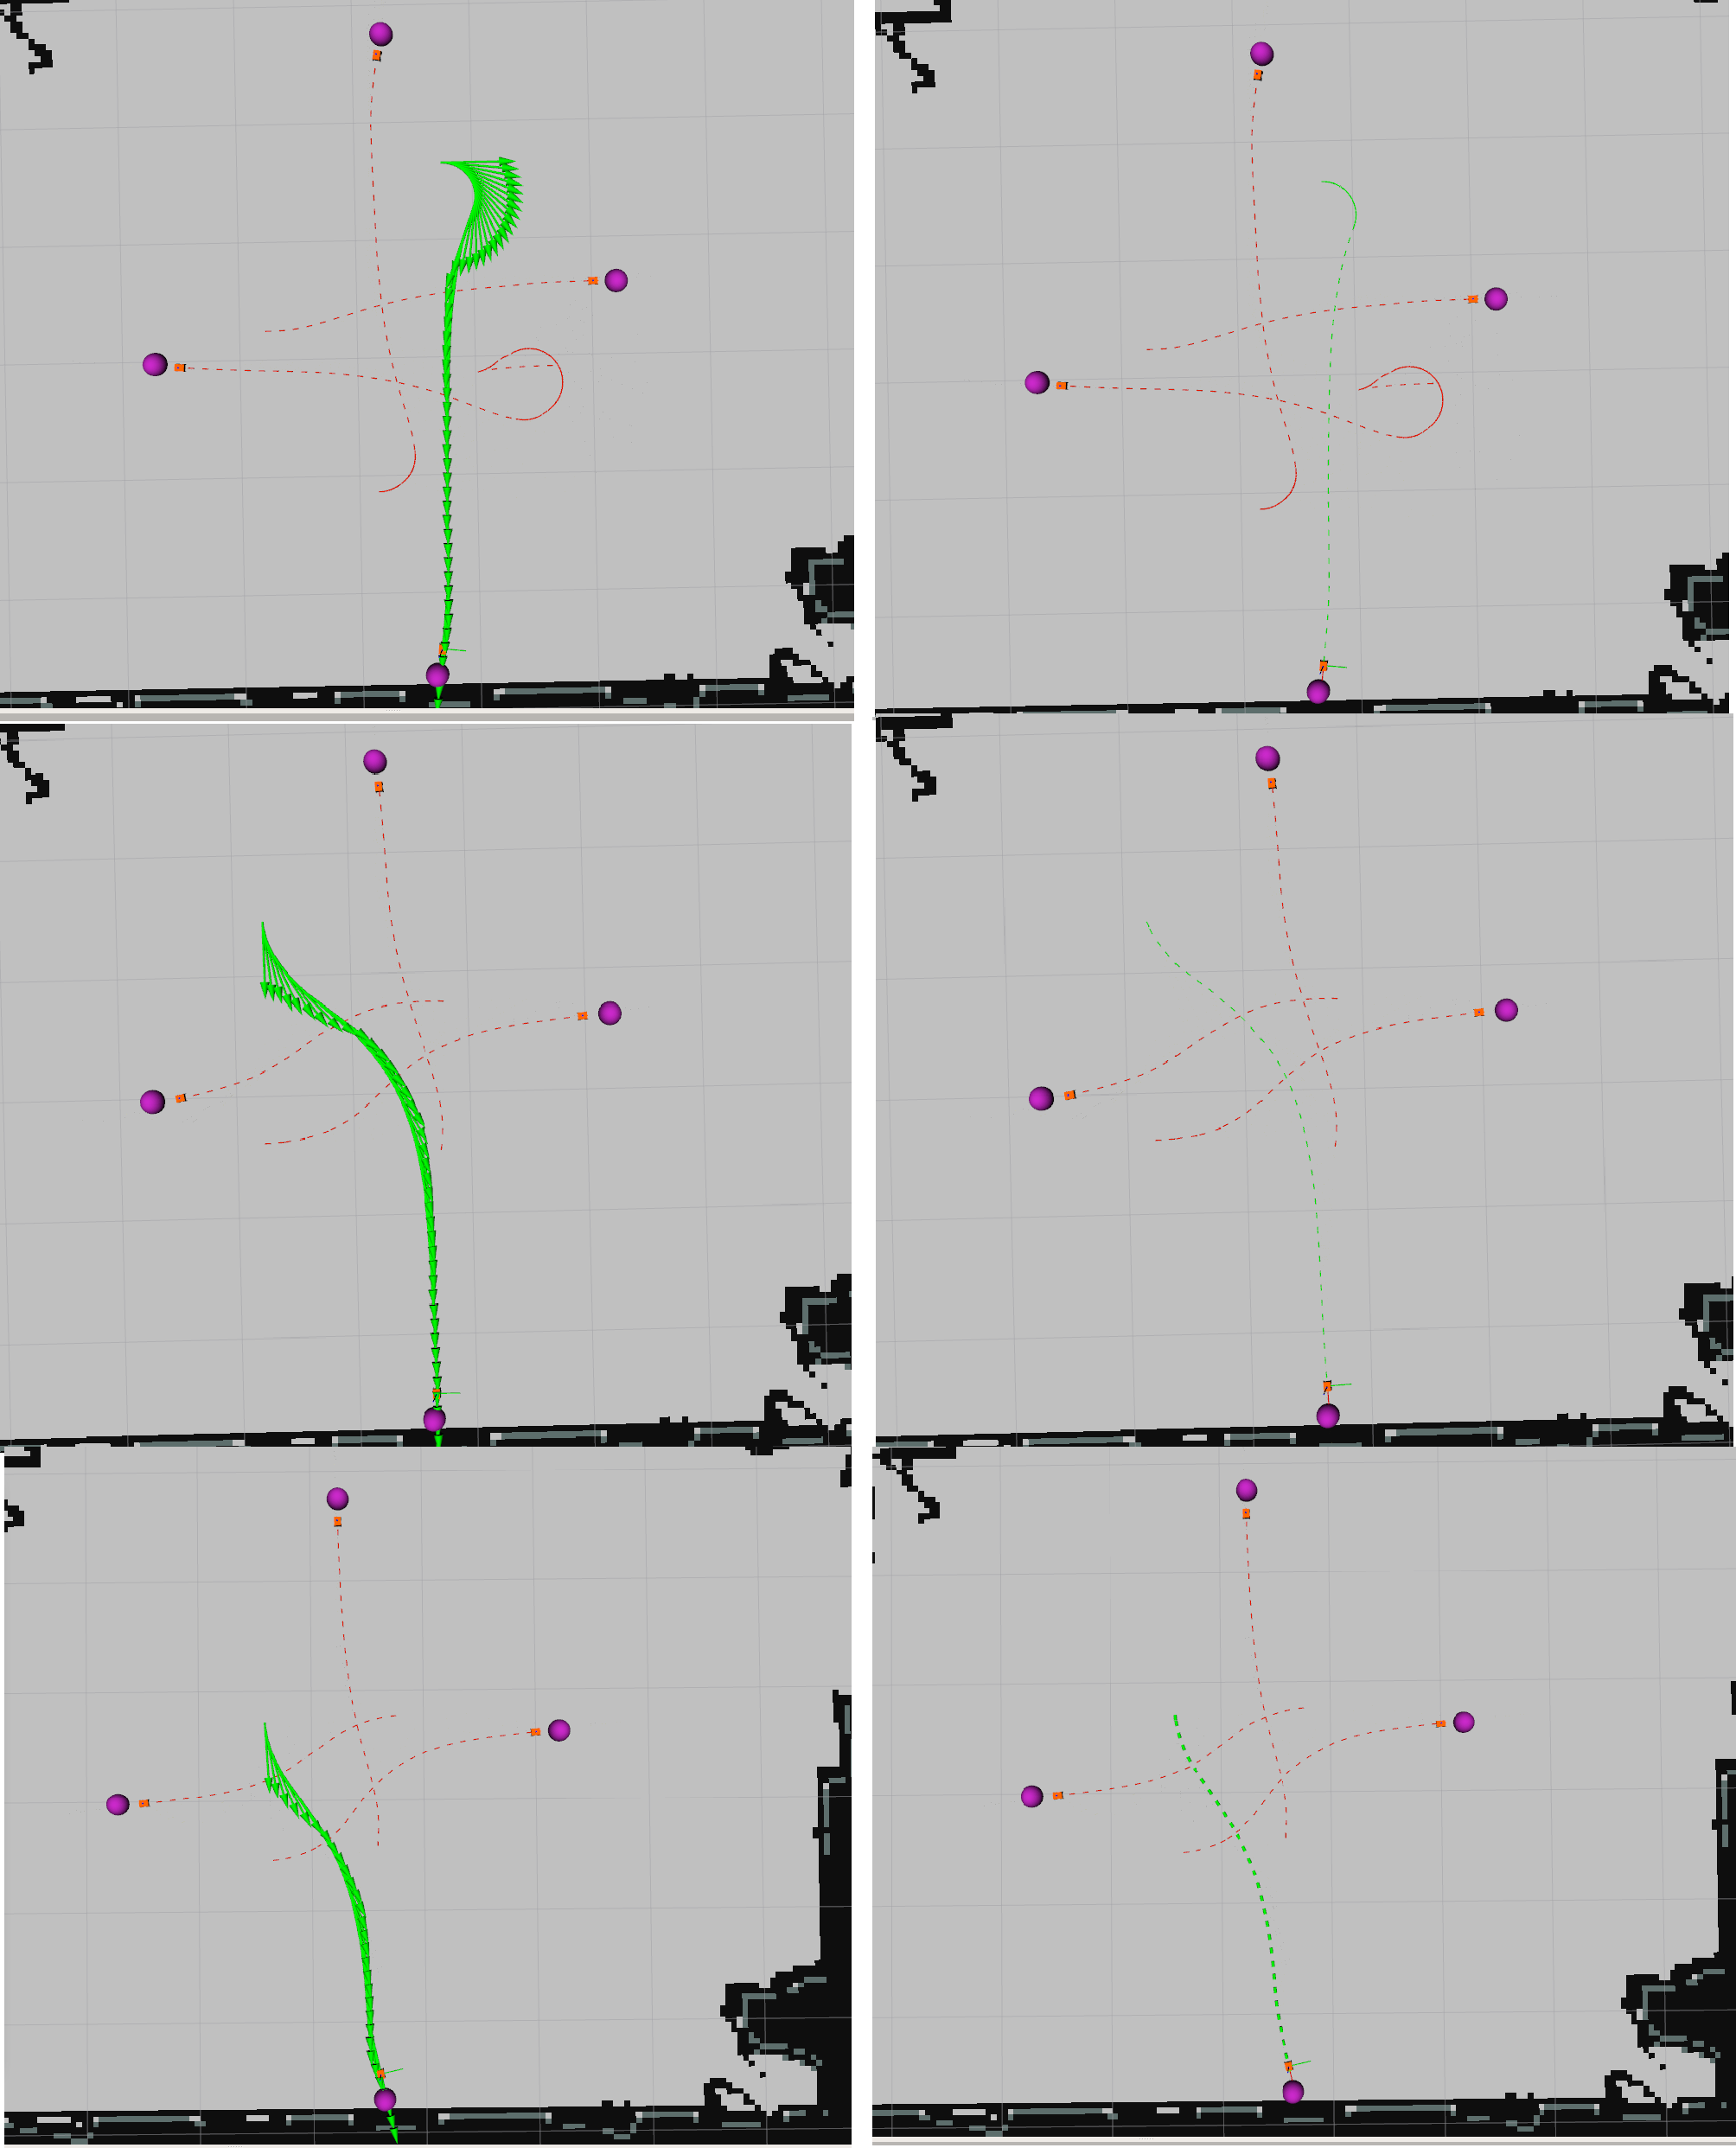
\includegraphics[scale=0.32]{orca_4_2.png}
    \caption{4动态障碍物对穿实验2(左边表示速度方向变化,右边表示最终轨迹)}
\end{figure}
此实验结果中包含了车头朝向不指向目标点等的情况,
从对穿实验可以看出,算法规划出的轨迹总是可以无碰撞且最优地到达对面目标点,无论阿克曼的模型处于什么样的状态和朝向。并且在运动过程中会根据实际情况实时调整速度的方向。

\subsubsection{争点穿插实验}
让4动态物体同向出发,向着对面的移动障碍物方向进发,过程中会出现动态障碍物从侧边出现的各种情况,实验结果展示如下:

\begin{figure}[ht]
    \centering
    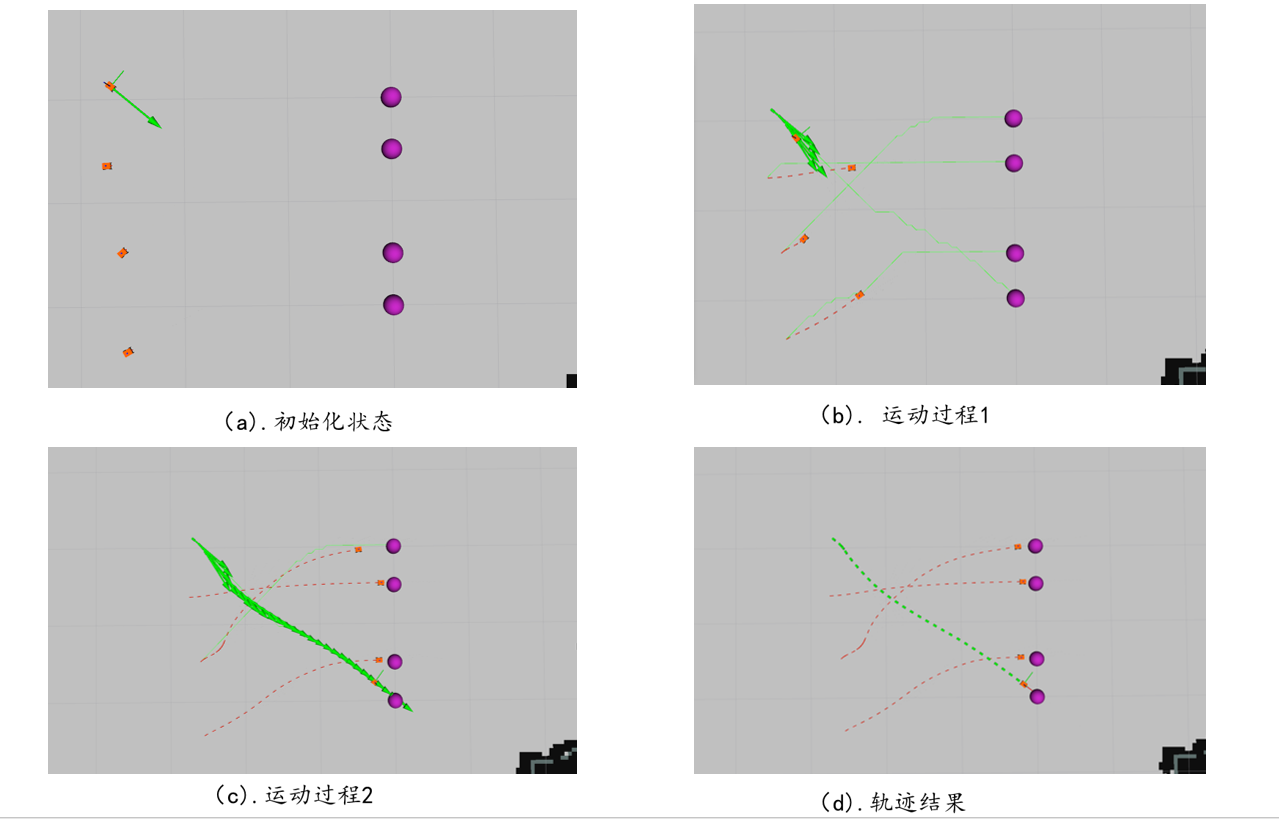
\includegraphics[scale=0.5]{orca_4_3.png}
    \caption{4动态障碍物争点穿插实验1}
\end{figure}

上图中的(b)、(c)图可以明显从速度的方向指向变化中感受到ORCA算法模块对移动机器人的速度调整,以避免即将到来的与其他移动机器人发生碰撞。

下图展示更多的实验结果以及将目标点数量减少,增加碰撞几率的实验结果。
\begin{figure}[ht]
    \centering
    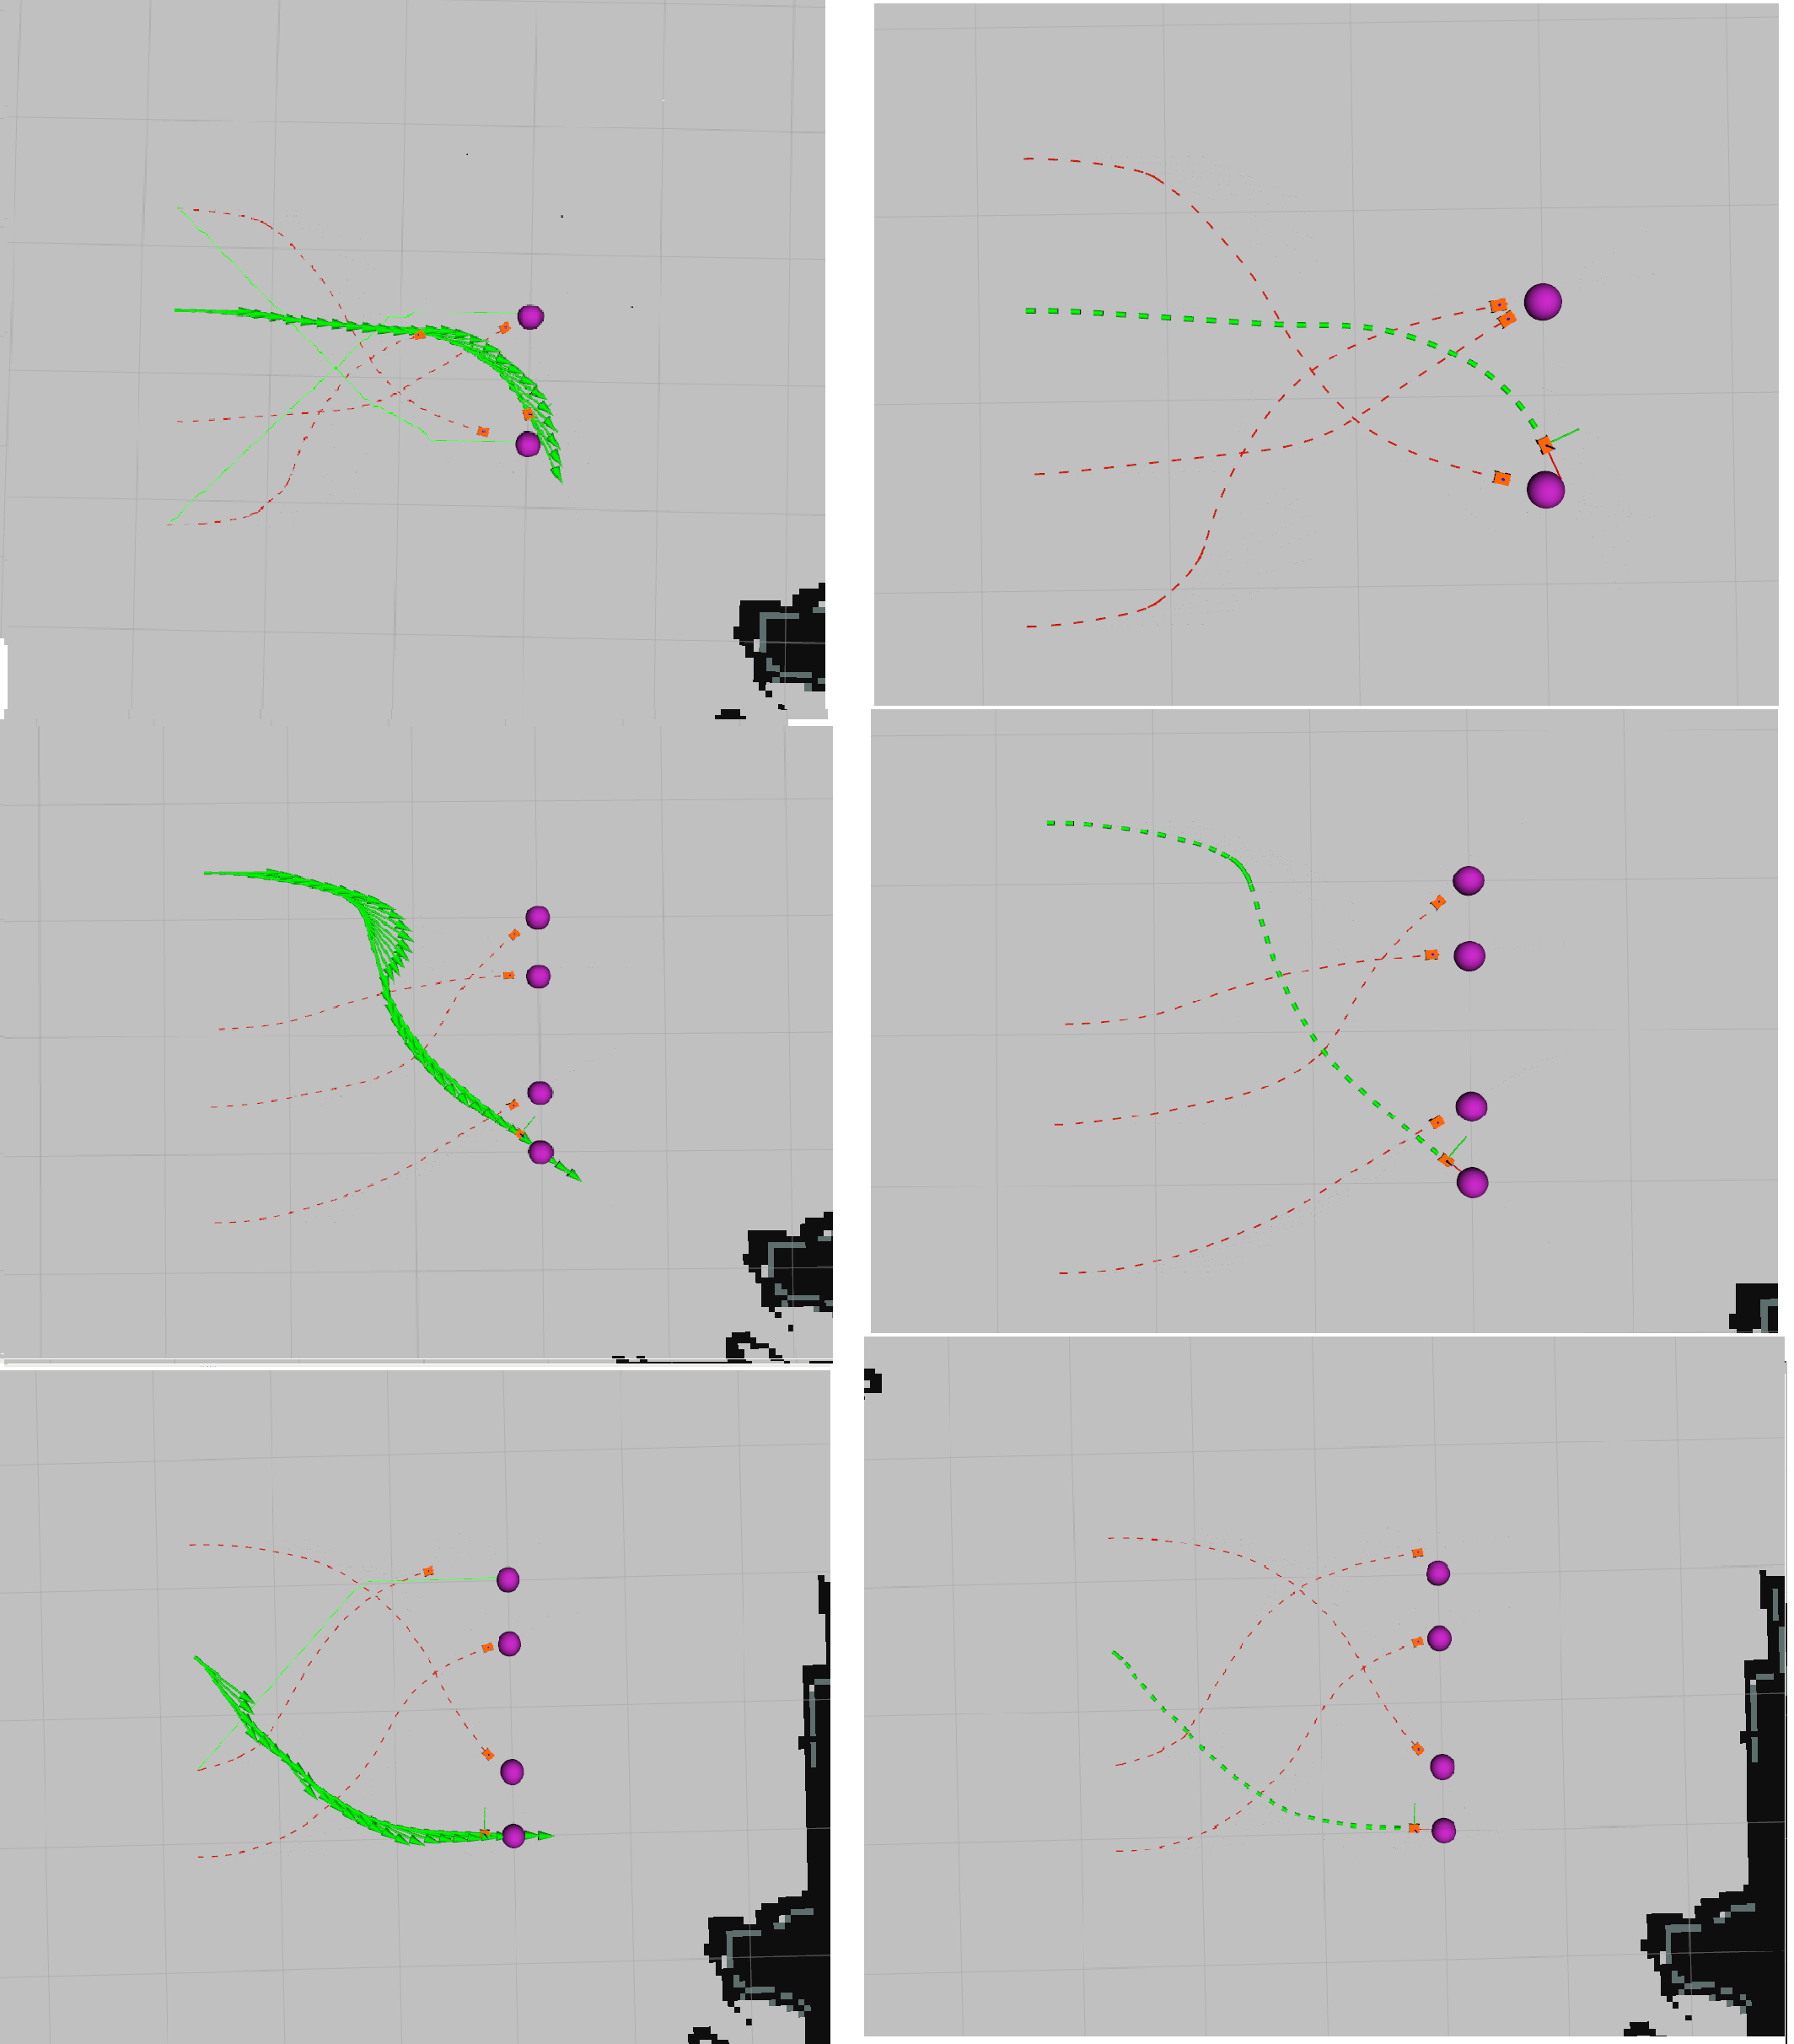
\includegraphics[scale=0.32]{orca_4_4.png}
    \caption{4动态障碍物争点穿插实验2(左边表示速度方向变化,右边表示最终轨迹)}
\end{figure}



\subsection{实验二:8动态障碍物遭遇实验}
实验在同一无静态障碍物区域放置8个动态物体,此8物体即互相做障碍物也单独可称为研究主体,增多动态障碍物数量,可加大对算法的考研难度,具体做法类似实验一,此处展示实验的结果轨迹。

\subsubsection{对穿实验}
\begin{figure}[ht]
    \centering
    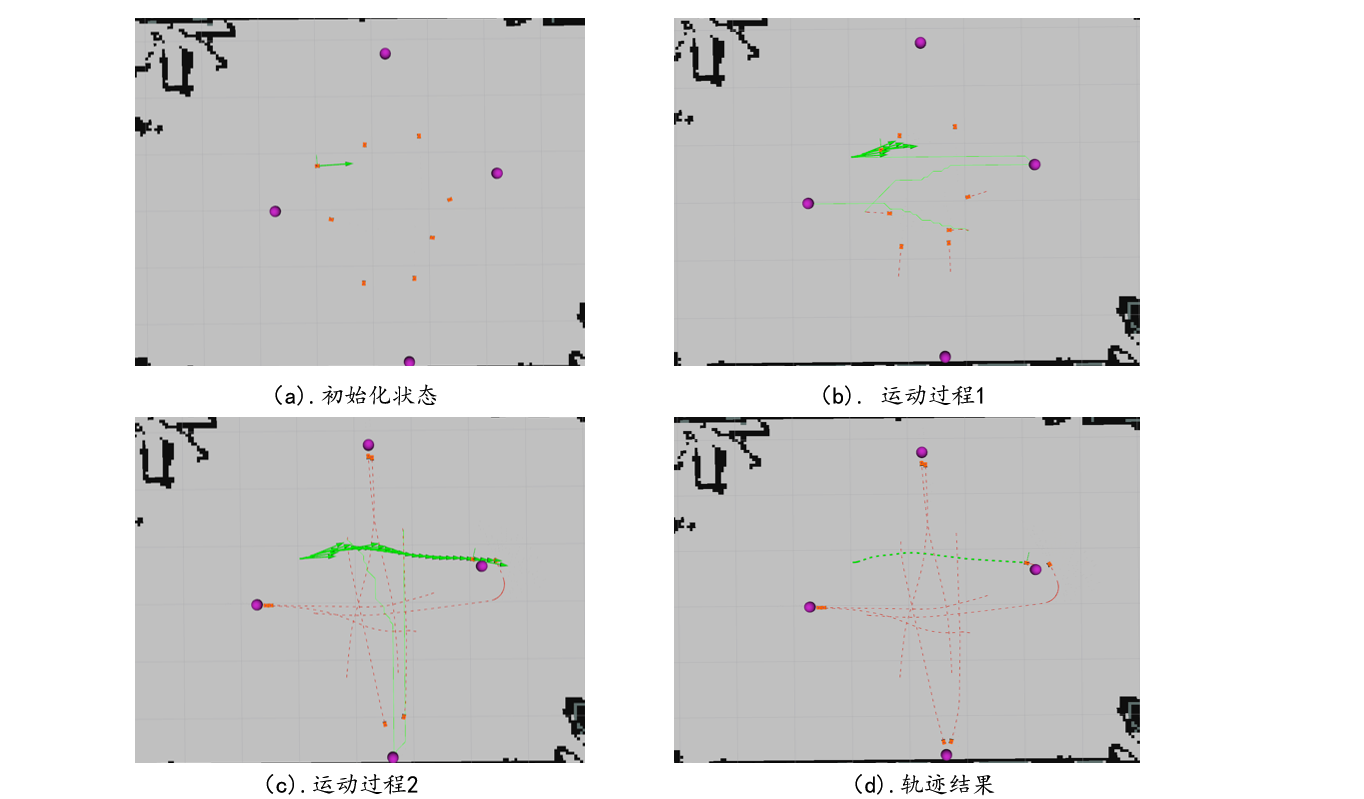
\includegraphics[scale=0.5]{orca_8_1.png}
    \caption{8动态障碍物对穿实验1}
\end{figure}
由上图可以看出,增加了动态障碍物之后,移动机器人的路径规划显然难度大幅增加,图中目标点在右侧的两个移动机器人中的红色轨迹明显看出由于计算出实验选定的对象的速度与当前速度相冲,有明显的转向避让趋势。

下面的实验结果展示更多的为运动过程中选定的对象的速度变化与最终轨迹,不再展示相应的运动过程。
\begin{figure}[ht]
    \centering
    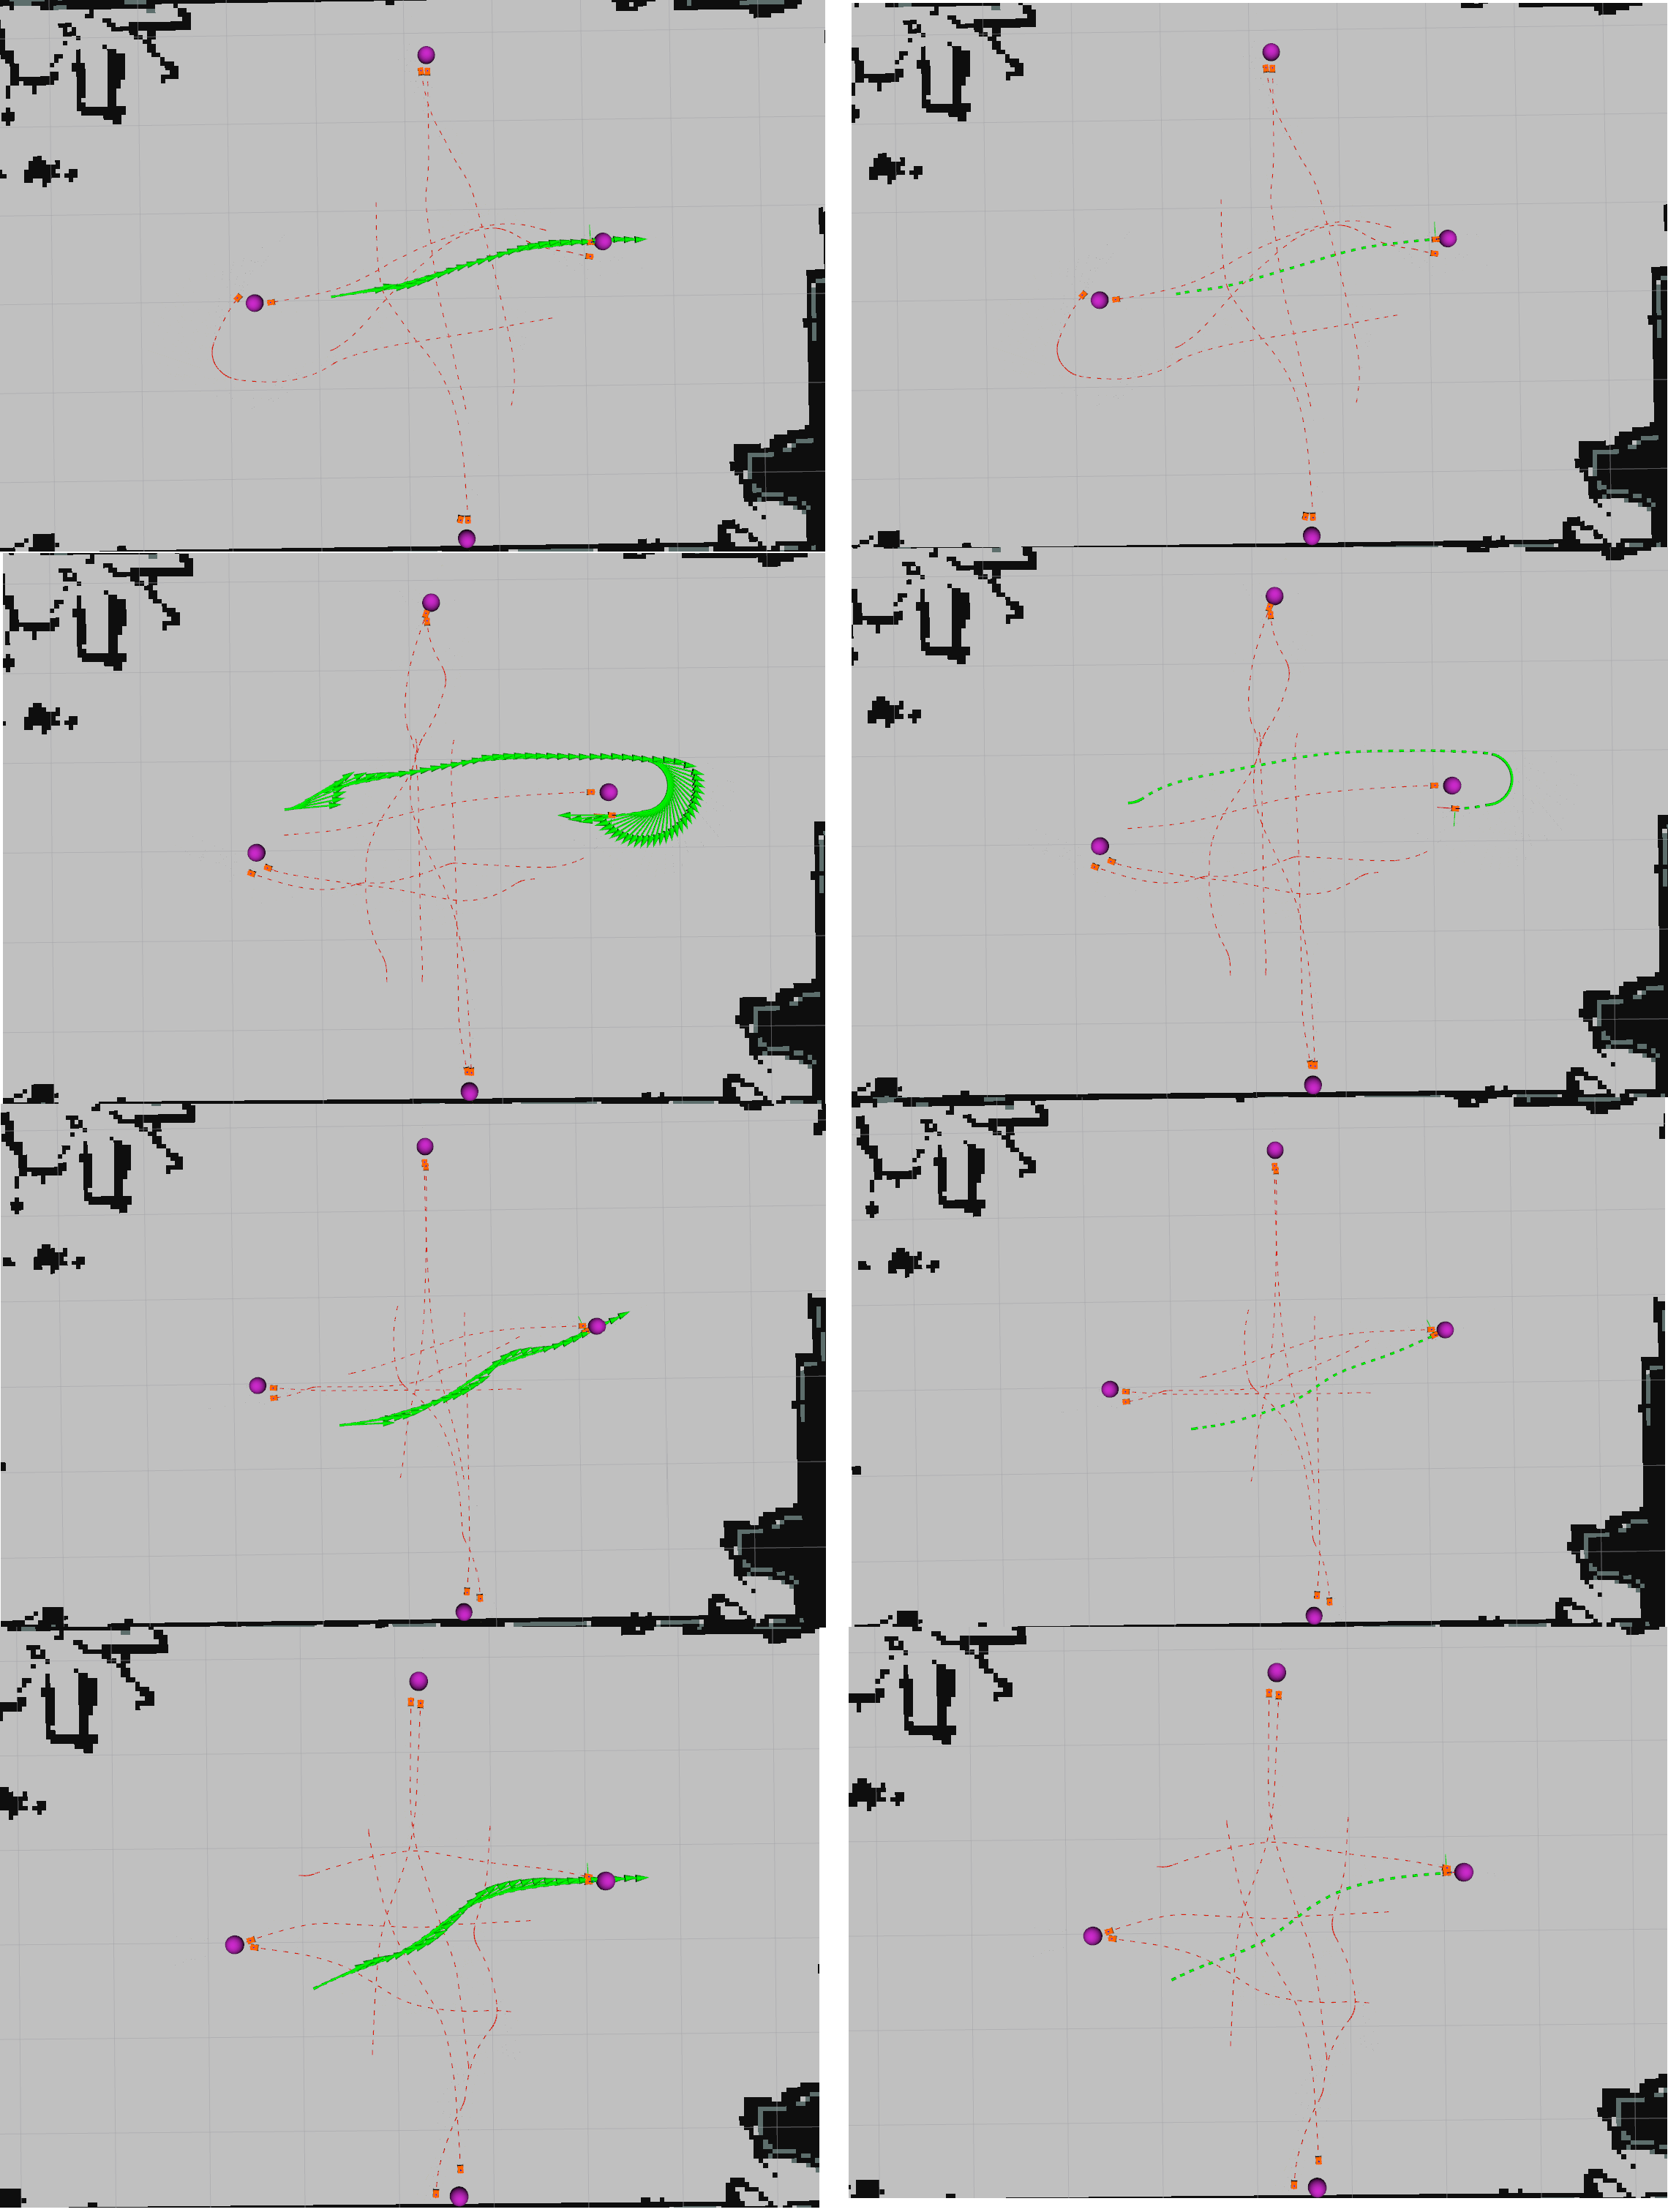
\includegraphics[scale=0.30]{orca_8_2.png}
    \caption{8动态障碍物对穿实验2(左边图片为选定对象的速度变化,右边为对对应的轨迹图)}
\end{figure}
通过8个动态障碍物的对穿实验可以看出,即使增加动态物后导致规划难度大大增加,但是本文提出的算法依然可以无碰撞且最优地规划出相应路径,并指引机器人到达目标点。


\subsubsection{争点穿插实验}
争点穿插实验为增大对算法的 考验力度,依然保持目标点的个数不变,此举动会大大增加移动物体之间的碰撞几率,穿插实验的目标点位置设置以及运动过程如下所示:

\begin{figure}[ht]
    \centering
    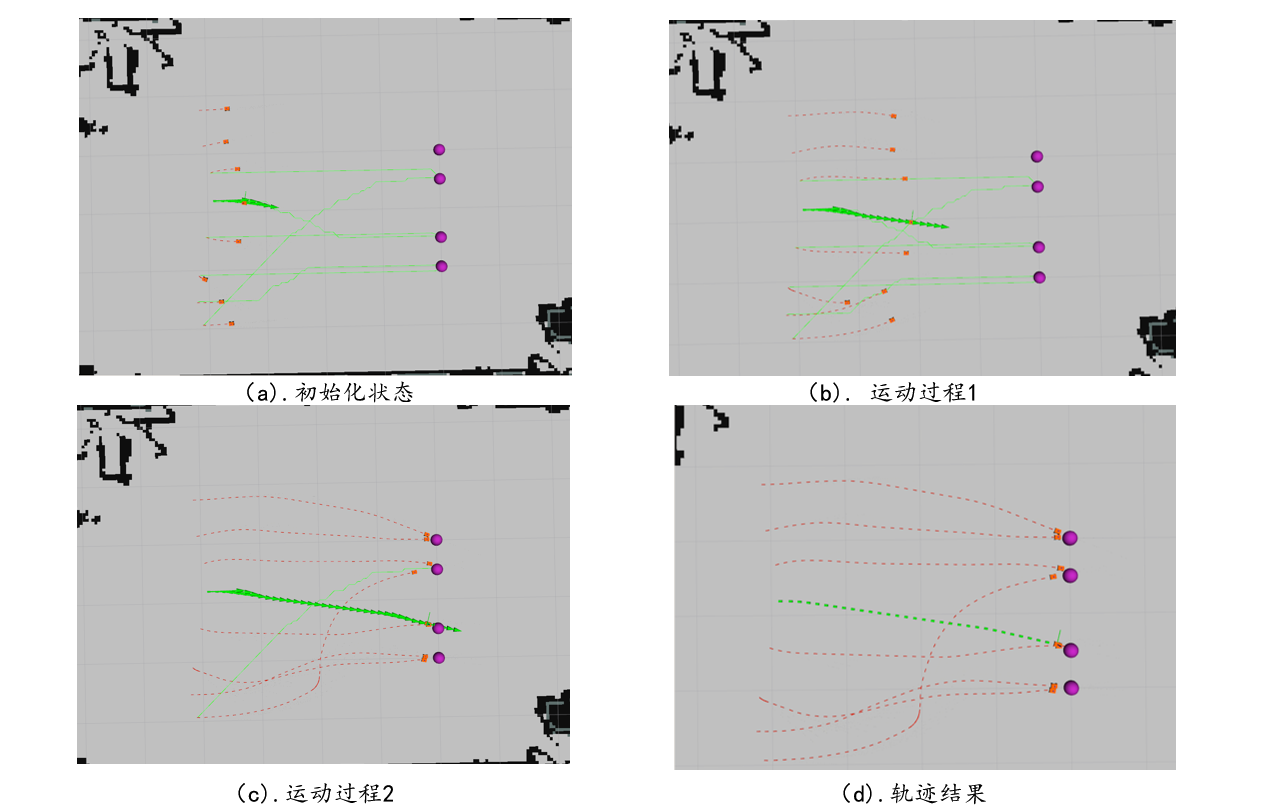
\includegraphics[scale=0.5]{orca_8_3.png}
    \caption{8动态障碍物争点穿插实验1}
\end{figure}
本图片中展示的轨迹规划结果可明显看出,移动机器人虽有A*算法规划出全局轨迹,但在多个移动障碍物的速度障碍阻拦下,不得不调整当前行驶路径以避免碰撞,这便是本文提出的算法调控的结果。

以下实验结果将更多展示8动态障碍物之间的争点穿插结果,并且下面实验中将目标点数量调整至2个点,在哪增加动态障碍物数量的基础上,增加全局A*算法在地图上规划出的轨迹密集度,实验结果展示如下:

\begin{figure}[ht]
    \centering
    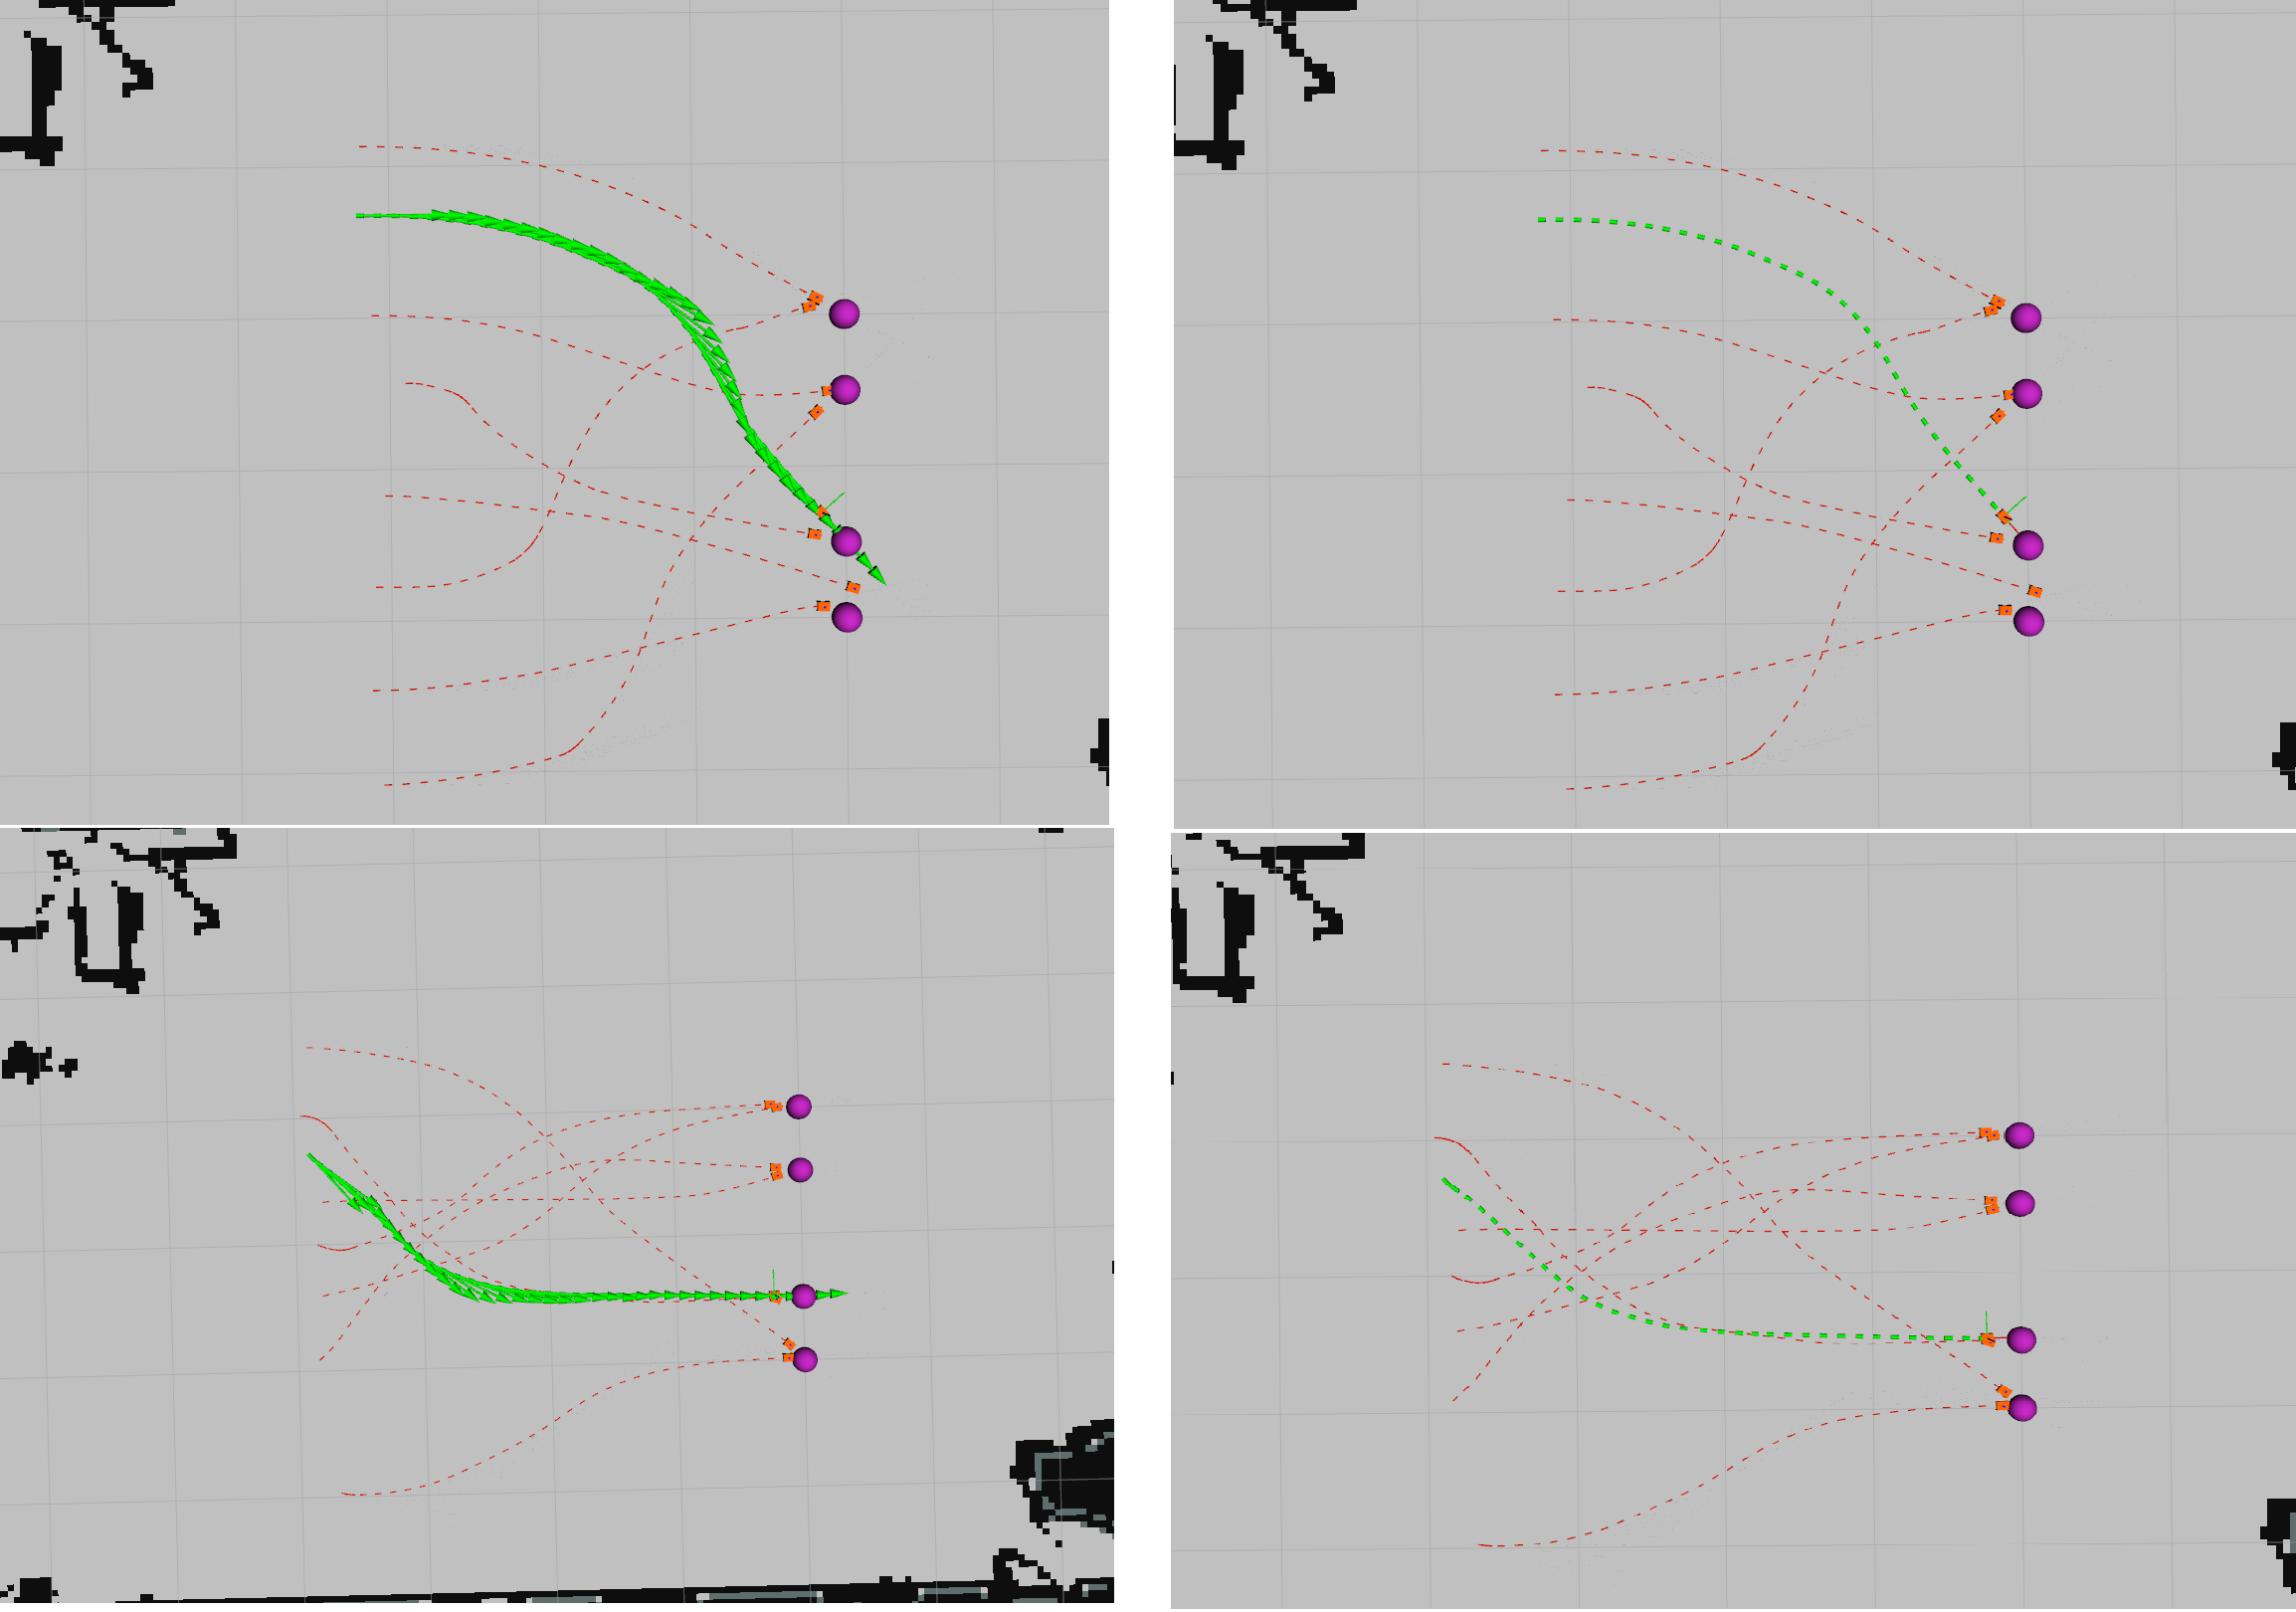
\includegraphics[scale=0.28]{orca_8_4.png}
    \caption{8动态障碍物争点穿插实验2(4目标点)}
\end{figure}

下面展示仅有两个目标点情况下的实验结果:
\begin{figure}[ht]
    \centering
    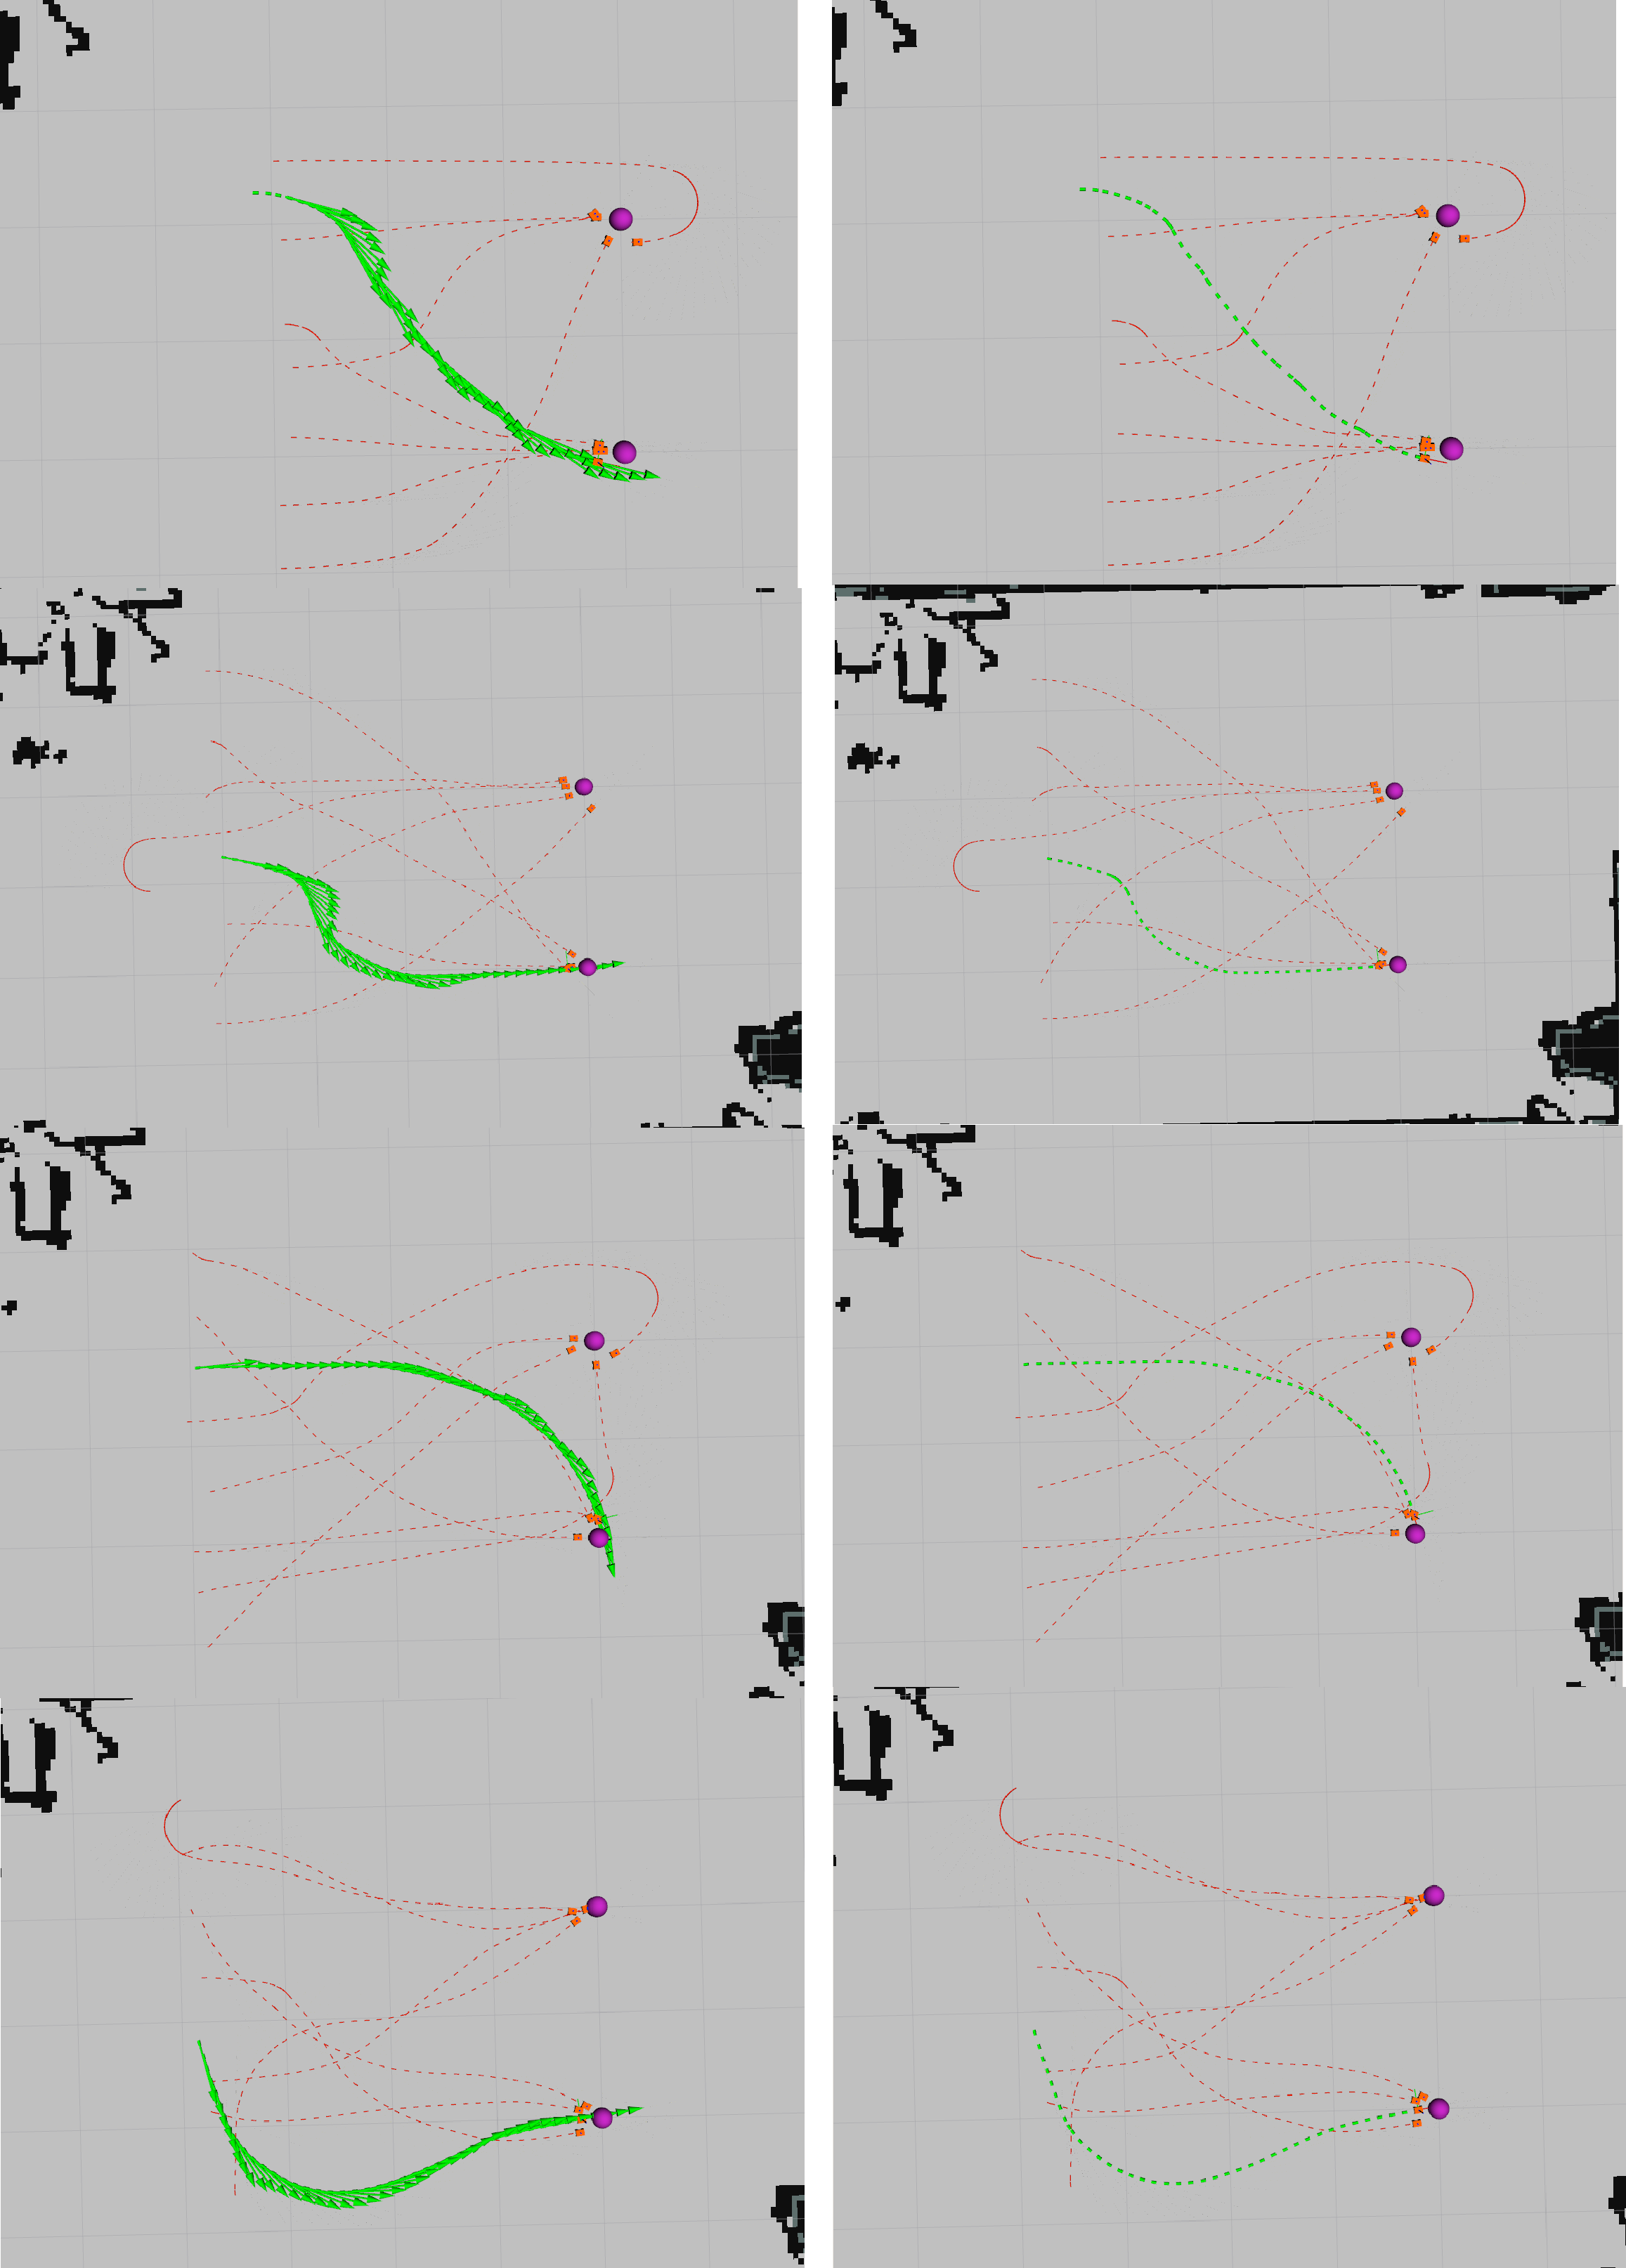
\includegraphics[scale=0.28]{orca_8_5.png}
    \caption{8动态障碍物争点穿插实验2(2目标点)}
\end{figure}


经过以上两轮多次实验,从实验结果中的速度变化以及轨迹图可以得出结论,本文提出的避障算法在和导航系统框架结合后可发挥出良好的动态避障效果。


\section{动态避障系统的实际场景实验}